\documentclass[a4paper, 12pt]{article}
% packages
\usepackage{amssymb}
\usepackage[fleqn]{mathtools}
\usepackage{tikz}
\usepackage{enumerate}
\usepackage{bussproofs}
\usepackage{xcolor}
\usepackage[margin=1.3cm]{geometry}
\usepackage{logicproof}
\usepackage{diagbox}
\usepackage{listings}
\usepackage{graphicx}
\usepackage{lstautogobble}
\usepackage{hyperref}
\usepackage{multirow}
\usepackage{tipa}
\usetikzlibrary{decorations.pathreplacing, arrows, shapes.gates.logic.US, circuits.logic.US, calc, automata, positioning}

% shorthand for verbatim
% this clashes with logicproof, so maybe fix this at some point?
\catcode`~=\active
\def~#1~{\texttt{#1}}

% code listing
\lstdefinestyle{main}{
    numberstyle=\tiny,
    breaklines=true,
    showspaces=false,
    showstringspaces=false,
    tabsize=2,
    numbers=left,
    basicstyle=\ttfamily,
    columns=fixed,
    fontadjust=true,
    basewidth=0.5em,
    autogobble,
    xleftmargin=3.0ex,
    mathescape=true
}
\newcommand{\dollar}{\mbox{\textdollar}} %
\lstset{style=main}

% augmented matrix
\makeatletter
\renewcommand*\env@matrix[1][*\c@MaxMatrixCols c]{%
\hskip -\arraycolsep
\let\@ifnextchar\new@ifnextchar
\array{#1}}
\makeatother

% ceiling / floor
\DeclarePairedDelimiter{\ceil}{\lceil}{\rceil}
\DeclarePairedDelimiter{\floor}{\lfloor}{\rfloor}

% custom commands
\newcommand{\indefint}[2]{\int #1 \, \mathrm{d}#2}
\newcommand{\defint}[4]{\int_{#1}^{#2} #3 \, \mathrm{d}#4}
\newcommand{\pdif}[2]{\frac{\partial #1}{\partial #2}}
\newcommand{\dif}[2]{\frac{\mathrm{d}#1}{\mathrm{d}#2}}
\newcommand{\limit}[2]{\raisebox{0.5ex}{\scalebox{0.8}{$\displaystyle{\lim_{#1 \to #2}}$}}}
\newcommand{\summation}[2]{\sum\limits_{#1}^{#2}}
\newcommand{\intbracket}[3]{\left[#3\right]_{#1}^{#2}}
\newcommand{\ulsmash}[1]{\underline{\smash{#1}}}

\newcommand{\powerset}[0]{\wp}
\renewcommand{\emptyset}[0]{\varnothing}

\makeatletter
\newsavebox{\@brx}
\newcommand{\llangle}[1][]{\savebox{\@brx}{\(\m@th{#1\langle}\)}%
  \mathopen{\copy\@brx\kern-0.5\wd\@brx\usebox{\@brx}}}
\newcommand{\rrangle}[1][]{\savebox{\@brx}{\(\m@th{#1\rangle}\)}%
  \mathclose{\copy\@brx\kern-0.5\wd\@brx\usebox{\@brx}}}
\makeatother
\newcommand{\lla}{\llangle}
\newcommand{\rra}{\rrangle}
\newcommand{\la}{\langle}
\newcommand{\ra}{\rangle}

\newcommand{\mat}[1]{\boldsymbol{#1}}
\renewcommand{\vec}[1]{\boldsymbol{#1}}
\newcommand{\rowt}[1]{\begin{bmatrix}
    #1
\end{bmatrix}^\top}

\newcommand{\unaryproof}[2]{\AxiomC{#1} \UnaryInfC{#2} \DisplayProof}
\newcommand{\binaryproof}[3]{\AxiomC{#1} \AxiomC{#2} \BinaryInfC{#3} \DisplayProof}
\newcommand{\trinaryproof}[4]{\AxiomC{#1} \AxiomC{#2} \AxiomC{#3} \TrinaryInfC{#4} \DisplayProof}

\newcommand{\axiom}[1]{\AxiomC{#1}}
\newcommand{\unary}[1]{\UnaryInfC{#1}}
\newcommand{\binary}[1]{\BinaryInfC{#1}}
\newcommand{\trinary}[1]{\TrinaryInfC{#1}}
\newcommand{\quaternary}[1]{\QuaternaryInfC{#1}}
\newcommand{\quinary}[1]{\QuinaryInfC{#1}}
\newcommand{\dproof}[0]{\DisplayProof}

\newcommand{\bnfsep}[0]{\ |\ }
\newcommand{\concsep}[0]{\ ||\ }
\newcommand{\violet}[1]{\textcolor{violet}{#1}}
\newcommand{\blue}[1]{\textcolor{blue}{#1}}
\newcommand{\red}[1]{\textcolor{red}{#1}}

% no indent
\setlength\parindent{0pt}

% reasoning proofs
\usepackage{ltablex}
\usepackage{environ}
\keepXColumns
\NewEnviron{reasoning}{
    \begin{tabularx}{\textwidth}{rlX}
        \BODY
    \end{tabularx}
}
\newcommand{\proofline}[3]{$(#1)$ & $#2$ & \hfill #3 \smallskip \\}
\newcommand{\proofarbitrary}[1]{& take arbitrary $#1$ \smallskip \\}
\newcommand{\prooftext}[1]{\multicolumn{3}{l}{#1} \smallskip \\}
\newcommand{\proofmath}[3]{$#1$ & = $#2$ & \hfill #3 \smallskip \\}
\newcommand{\prooftherefore}[1]{& $\therefore #1$ \smallskip \\}
\newcommand{\proofbc}[0]{\prooftext{\textbf{Base Case}}}
\newcommand{\proofis}[0]{\prooftext{\textbf{Inductive Step}}}

% reasoning er diagrams
\newcommand{\nattribute}[4]{
    \node[draw, state, inner sep=0cm, minimum size=0.2cm, label=#3:{#4}] (#1) at (#2) {};
}
\newcommand{\mattribute}[4]{
    \node[draw, state, accepting, inner sep=0cm, minimum size=0.2cm, label=#3:{#4}] (#1) at (#2) {};
}
\newcommand{\dattribute}[4]{
    \node[draw, state, dashed, inner sep=0cm, minimum size=0.2cm, label=#3:{#4}] (#1) at (#2) {};
}
\newcommand{\entity}[3]{
    \node[] (#1-c) at (#2) {#3};
    \node[inner sep=0cm] (#1-l) at ($(#1-c) + (-1, 0)$) {};
    \node[inner sep=0cm] (#1-r) at ($(#1-c) + (1, 0)$) {};
    \node[inner sep=0cm] (#1-u) at ($(#1-c) + (0, 0.5)$) {};
    \node[inner sep=0cm] (#1-d) at ($(#1-c) + (0, -0.5)$) {};
    \draw
    ($(#1-c) + (-1, 0.5)$) -- ($(#1-c) + (1, 0.5)$) -- ($(#1-c) + (1, -0.5)$) -- ($(#1-c) + (-1, -0.5)$) -- cycle;
}
\newcommand{\relationship}[3]{
    \node[] (#1-c) at (#2) {#3};
    \node[inner sep=0cm] (#1-l) at ($(#1-c) + (-1, 0)$) {};
    \node[inner sep=0cm] (#1-r) at ($(#1-c) + (1, 0)$) {};
    \node[inner sep=0cm] (#1-u) at ($(#1-c) + (0, 1)$) {};
    \node[inner sep=0cm] (#1-d) at ($(#1-c) + (0, -1)$) {};
    \draw
    ($(#1-c) + (-1, 0)$) -- ($(#1-c) + (0, 1)$) -- ($(#1-c) + (1, 0)$) -- ($(#1-c) + (0, -1)$) -- cycle;
}

% actual document
\begin{document}
    \section*{CO233 - Computational Techniques}
        \subsection*{15th January 2020}
            \subsubsection*{Vector and Matrix Norms}
                An orthonormal basis of $\mathbb{R}^n$ are unit vectors that are pairwise mutually perpendicular; such that for $(e_1, \cdots, e_n)$;
                \begin{itemize}
                    \itemsep0em
                    \item $e_i \cdot e_i = 1$
                    \item $e_i \cdot e_j = 0$, if $i \neq j$
                \end{itemize}
                The standard canonical basis of $\mathbb{R}^3$ are the $i,j,k$ vectors, and similar in $\mathbb{R}^2$.
                However, we can form another orthonormal basis of $\mathbb{R}^2$ by bisecting the angles as such;
                \begin{center}
                    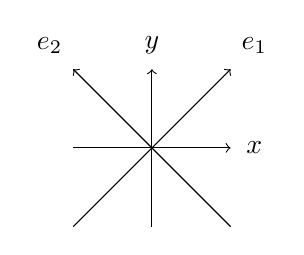
\begin{tikzpicture}
                        \node (y) at (0, 1.3) {$y$};
                        \node (x) at (1.3, 0) {$x$};
                        \node (e1) at (1.3, 1.3) {$e_1$};
                        \node (e2) at (-1.3, 1.3) {$e_2$};
                        \draw
                        (0, -1) edge[->] (0, 1)
                        (-1, 0) edge[->] (1, 0)
                        (-1, -1) edge[->] (1, 1)
                        (1, -1) edge[->] (-1, 1);
                    \end{tikzpicture}
                \end{center}
                If we take a vector $\vec{v} \in \mathbb{R}^n$, the Euclidean norm (or the $\ell_2$-norm) is defined as such;
                \begin{center}
                    $|| \vec{v} ||_2 = \sqrt{\summation{i=1}{n} v_i^2}$
                \end{center}
                A norm, a mapping $||\ || : \mathbb{R}^n \to \mathbb{R}^+$, must satisfy these 3 axioms;
                \begin{enumerate}[(i)]
                    \itemsep0em
                    \item $|| \vec{v} || > 0$ given that $\vec{v} \neq \vec{0}$
                    \item $|| \lambda \vec{v} || = |\lambda|\ || \vec{v} ||$
                    \item $|| \vec{v} + \vec{w} || \leq || \vec{v} || + || \vec{w} ||$ (triangular inequality)
                \end{enumerate}
                Some other ($\ell_p$) norms are defined as follows;
                \begin{align*}
                    \ell_1\text{-norm } || \vec{v} ||_1 & = \summation{i=1}{n}|v_i| \\
                    \ell_\infty\text{-norm } || \vec{v} ||_\infty & = \max \{|v_i| : 1 \leq i \leq n\} \\
                    \ell_p\text{-norm } || \vec{v} ||_p & = \left(\summation{i=1}{n} |v_i|^p\right)^\frac{1}{p}
                \end{align*}
                In each dimension, we have the following;
                \begin{itemize}
                    \itemsep0em
                    \item $n = 1$
                        \begin{itemize}
                            \itemsep0em
                            \item $|| \vec{v} ||_1 = | v | = | v |$
                            \item $|| \vec{v} ||_2 = \sqrt{v^2} = | v |$
                            \item $|| \vec{v} ||_\infty = \max \{| v |\} = | v |$
                        \end{itemize}
                    \item $n = 2$
                        \smallskip

                        We can represent this geometrically as such;
                        \begin{center}
                            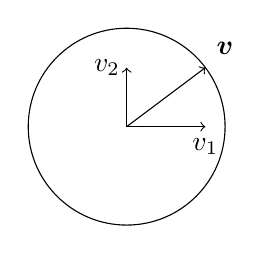
\begin{tikzpicture}[x=0.25cm, y=0.25cm]
                                \node at (4, -1) {$v_1$};
                                \node at (-1, 3) {$v_2$};
                                \node at (5, 4) {$\vec{v}$};

                                \draw (0, 0) circle (5);
                                \draw (0, 0) edge[->] (4, 0);
                                \draw (0, 0) edge[->] (0, 3);
                                \draw (0, 0) edge[->] (4, 3);
                            \end{tikzpicture}
                        \end{center}
                        In our case $|| \vec{v} ||_\infty = \max\{ | v_1 |, | v_2 | \} = | v_1 |$, but the point is that it's either of the "sides" of the triangle.
                        Obviously, $|| \vec{v} ||_2 \geq || \vec{v} ||_\infty$, as it's the hypotenuse of the triangle, and similarly, $|| \vec{v} ||_1 \geq || \vec{v} ||_2$, due to the triangle inequality.
                        Therefore we have $|| \vec{v} ||_1 \geq || \vec{v} ||_2 \geq || \vec{v} ||_\infty$.
                        \smallskip

                        Even if the orthonormal base changes, the Euclidean norm stays the same, whereas the other norms can change.
                        As such, we can say the $\ell_2$-norm is invariant under an \textbf{orthogonal transformation} (a basis change from an orthonormal bases to another orthonormal bases).
                    \item $n =\ ?$ (general)
                        \smallskip

                        The goal is to prove $|| \vec{v} ||_\infty \leq || \vec{v} ||_2 \leq || \vec{v} ||_1$.
                        If we first take the squares of all of them, such that we have the following;
                        \begin{align*}
                            || \vec{v} ||_1^2 & = \left(\summation{i = 1}{n} | v_i |\right)^2 \\
                            || \vec{v} ||_2^2 & = \summation{i = 1}{n} | v_i |^2 \\
                            || \vec{v} ||_\infty^2 & = (\max\{| v_i | : 1 \leq i \leq n\})^2 \\
                        \end{align*}
                        Since the $\ell_\infty$-norm corresponds to a single $v_i$, it's obvious that the following inequality holds (since the $\ell_2$-norm squared has all the other terms squared, as well as the $\ell_\infty$-norm squared);
                        \begin{center}
                            $|| \vec{v} ||_2^2 = \summation{i = 1}{n} | v_i |^2 \geq (\max\{| v_i | : 1 \leq i \leq n\})^2 = || \vec{v} ||_\infty^2 \Rightarrow || \vec{v} ||_2 \geq || \vec{v} ||_\infty$
                        \end{center}
                        To prove the other inequality, we see that the square of the sum of absolutes is greater than the sum of the squares, as the square of the sum contains the cross terms (which will be positive).
                        \begin{center}
                            $|| \vec{v} ||_2^2 = \summation{i = 1}{n} | v_i |^2 \leq \left(\summation{i = 1}{n} | v_i |\right)^2 = || \vec{v} ||_\infty^1 \Rightarrow || \vec{v} ||_2 \leq || \vec{v} ||_1$
                        \end{center}
                        As such, we can conclude that $|| \vec{v} ||_\infty \leq || \vec{v} ||_2 \leq || \vec{v} ||_1$ in any dimension. \hfill $\blacksquare$
                \end{itemize}
            \subsubsection*{Tutorial Question}
                Find the locus of vectors such that $|| \vec{v} ||_p \leq 1$, for $p = \red{1}, \blue{2}, \violet{\infty}$ in $n = 2$;
                \begin{center}
                    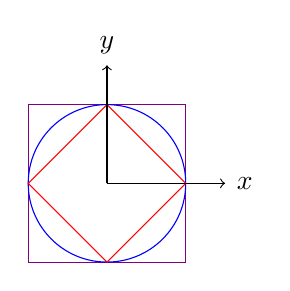
\begin{tikzpicture}
                        \node at (1.75, 0) {$x$};
                        \node at (0, 1.75) {$y$};

                        \draw[violet] (-1, 1) -- (1, 1) -- (1, -1) -- (-1, -1) -- cycle;
                        \draw[blue] (0, 0) circle (1);
                        \draw[red] (0, 1) -- (1, 0) -- (0, -1) -- (-1, 0) -- cycle;
                        \draw
                        (0, 0) edge[->] (1.5, 0)
                        (0, 0) edge[->] (0, 1.5);
                    \end{tikzpicture}
                \end{center}
                Imagine they're all shaded from the border to the origin.
            \subsubsection*{$\ell_p$-norm}
                Our goal is to show that as $p \to \infty$, we get the definition of the $\ell_\infty$-norm previously stated.
                Take a vector $\vec{v} \in \mathbb{R}^n$, where both $\vec{v}$ and $n$ are fixed.
                \begin{center}
                    $|| \vec{v} ||_p^p = \summation{i = 1}{n} | v_i |^p$
                \end{center}
                Obviously, this is greater than or equal to $|| \vec{v} ||_\infty^p$, as it would only be a single $| v_i |^p$.
                Similarly, it must be less than or equal to $n | v_i |^p$, as $v_i$ is the maximum of all the components.
                \begin{center}
                    $|| \vec{v} ||_\infty^p \leq || \vec{v} ||_p^p = \summation{i = 1}{n} | v_i |^p \leq n || \vec{v} ||_\infty^p$
                \end{center}
                Taking everything to the power of $\frac{1}{p}$, we obtain the following result (note that $p > 0$ hence the signs don't change);
                \begin{center}
                    $|| \vec{v} ||_\infty \leq || \vec{v} ||_p = \leq n^\frac{1}{p} || \vec{v} ||_\infty$
                \end{center}
                As $p \to \infty$, since $n \geq 2$ ($n = 1$ is shown to collapse to the same component), we have $n^\frac{1}{p} \to 1$, which sandwiches the middle term.
            \subsubsection*{Some Proposition ($\ell_\infty$-norm vs $\ell_2$-norm)}
                The proposition is as follows; for a vector $\vec{v} \in \mathbb{R}^n$, $|| \vec{v} ||_2 \leq \sqrt{n} || \vec{v} ||_\infty$.
                To show this, we know that each of $| v_i |$ is less than or equal to $|| \vec{v} ||_\infty$, by definition of the maximum.
                The same can be said for $| v_i |^2$, vs $|| \vec{v} ||_\infty^2$.
                Taking square roots, we have the following;
                \begin{center}
                    $|| \vec{v} ||_2^2 = \summation{i = 1}{n} | v_i |^2 \leq n || \vec{v} ||_\infty^2 \Rightarrow || \vec{v} ||_2 \leq \sqrt{n} || \vec{v} ||_\infty$
                \end{center}
                To show this holds similarly for $|| \vec{v} ||_1 \leq \sqrt{n} || \vec{v} ||_2$, we employ the Cauchy-Schwarz inequality, which states $| \vec{x} \cdot \vec{y} | \leq || \vec{x} ||_2 || \vec{y} ||_2$.
                The Cauchy-Schwarz inequality uses the fact that $\vec{x} \cdot \vec{y} = || \vec{x} ||_2 || \vec{y} ||_2 \cos \theta$.
                To do this, we need to define a sign function $\text{sgn} : \mathbb{R} \to \{1, -1\}$ as follows;
                \begin{align*}
                    \text{sgn}\ x & = \begin{cases}
                        1 & x \geq 0 \\
                        -1 & x < 0
                    \end{cases}
                    \intertext{We also need to craft a vector $\vec{w}$, as follows;}
                    w_i & = \frac{\text{sgn}\ v_i}{\sqrt{n}} & 1 \leq i \leq n \\
                    \vec{v} \cdot \vec{w} & = \summation{i = 1}{n} v_i w_i \\
                    & = \summation{i = 1}{n} \frac{v_i \cdot \text{sgn}\ v_i}{\sqrt{n}} & \text{product of same sign becomes positive} \\
                    & = \summation{i = 1}{n} \frac{| v_i |}{\sqrt{n}} \\
                    & = \sqrt{n} \summation{i = 1}{n} | v_i | \\
                    & = \sqrt{n} || \vec{v} ||_1 \\
                    || \vec{w} ||_2 & = \summation{i = 1}{n} \frac{\pm 1}{\sqrt{n}}^2 \\
                    & = \summation{i = 1}{n} \frac{1}{n} \\
                    & = 1
                \end{align*}
                By \violet{Cauchy-Schwarz}, we get;
                \begin{center}
                    $\sqrt{n} || \vec{v} ||_1 = \violet{| \vec{v} \cdot \vec{w} | \leq || \vec{v} ||_2 || \vec{w} ||_2} = || \vec{v} ||_2$
                \end{center}
        \subsection*{16th January 2020}
            Note that this recording has \textbf{no audio}, and therefore will just be the board transcribed.
            I honestly have no idea what he was doing in this lecture, it seems to just jump from topic to topic.
            \subsubsection*{Equivalence of Norms?}
                Take any two norms on $\mathbb{R}^n$; $||\ ||_a$, and $||\ ||_b$.
                \begin{center}
                    $\exists r, s \in \mathbb{R}^+\ \forall \vec{v} \in \mathbb{R}^n\ [r || \vec{v} ||_b \leq || \vec{v} ||_a \leq s || \vec{v} ||_b]$
                \end{center}
                This means that norms in finite dimensional vector spaces are equivalent (no idea why, look it up).
            \subsubsection*{Convergence of Vector Sequences}
                $(\vec{r}_n)$ is a sequence of vectors, and $(a_{i, j})$ is the $i, j^\text{th}$ entry of $\mat{A}$.
                For a vector $\vec{v}^{(m)} \in \mathbb{R}^n$, where $m = 0, 1, 2, \dots$
                \begin{align*}
                    \vec{v}^{(m)} & = \begin{bmatrix}
                        v_1^{(m)} \\ v_2^{(m)} \\ \vdots \\ v_n^{(m)}
                    \end{bmatrix}
                \end{align*}
                For a vector sequence $\vec{v}^{(m)}$ to converge to some vector $\vec{v} \in \mathbb{R}^n$, the following must hold;
                \begin{center}
                    $\vec{v}^{(m)} \to \vec{v} \in \mathbb{R}^n \Leftrightarrow \limit{m}{\infty} || \vec{v}^{(m)} - \vec{v} || \to 0$
                \end{center}
                This is componentwise convergence, such that $\forall i \in [1, n]\ [v_i^{(m)} \to v_i]$.
            \subsubsection*{Matrix Norms}
                Vectors are a type of matrix.
                For a matrix $\mat{A} \in \mathbb{R}^{m \times n}$, the following properties of its norms must hold, where $||\ || : \mathbb{R}^{m \times n} \to \mathbb{R}_{\geq 0}$;
                \begin{enumerate}[(i)]
                    \itemsep0em
                    \item $|| \mat{A} || > 0$ given that $\mat{A} \neq \mat{0}$
                    \item $|| \lambda \mat{A} || = | \lambda | || \mat{A} ||$
                    \item $|| \mat{A} + \mat{B} || \leq || \mat{A} || + || \mat{B} ||$
                    \item $|| \mat{B} \mat{A} || \leq || \mat{B} || || \mat{A} ||$
                \end{enumerate}
                \begin{center}
                    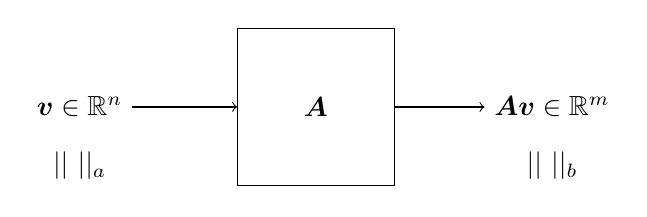
\begin{tikzpicture}
                        \node (v) at (0, 0) {$\vec{v} \in \mathbb{R}^n$};
                        \node at (0, -0.75) {$||\ ||_a$};
                        \node (av) at (6, 0) {$\mat{A} \vec{v} \in \mathbb{R}^m$};
                        \node at (6, -0.75) {$||\ ||_b$};
                        \node at (3, 0) {$\mat{A}$};
                        \draw
                        (v) edge[->] (2, 0)
                        (4, 0) edge[->] (av)
                        (2, 1) -- (4, 1) -- (4, -1) -- (2, -1) -- cycle;
                    \end{tikzpicture}
                    \medskip

                    $|| \mat{A} \vec{v} ||_b \leq || \mat{A} || || \vec{v} ||_a$
                \end{center}
                For the following example, take $(a_{i, j}) = \mat{A} \in \mathbb{R}^{m \times n}$;
                \begin{align*}
                    a_j & = \begin{bmatrix}
                        a_{1, j} \\ a_{2, j} \\ \vdots \\ a_{m, j}
                    \end{bmatrix} & \text{the $j^\text{th}$ column of $\mat{A}$} \\
                    a^i & = \begin{bmatrix}
                        a_{i, 1} & a_{i, 2} & \cdots & a_{i, n}
                    \end{bmatrix} & \text{the $i^\text{th}$ row of $\mat{A}$}
                \end{align*}
                We have the following norms on matrices;
                \begin{align*}
                    || \mat{A} ||_1 & = \max \{|| a_j ||_1 : 1 \leq j \leq n \} \\
                    || \mat{A} ||_\infty & = \max \{|| (a^i)^\top ||_1 : 1 \leq i \leq m \} \\
                    || \mat{A} ||_F & = \sqrt{\summation{i = 1}{m} \summation{j = 1}{n} | a_{i, j} |^2} & \text{Frobenius norm} \\
                    || \mat{A} ||_2 & = \text{largest singular value of } \mat{A} \\
                    \text{let } \mat{A} & = \begin{bmatrix}
                        2 & 3 & 1 & 4 \\
                        1 & 3 & -1 & 5 \\
                        \sqrt{2} & 0 & -2 & 2
                    \end{bmatrix} \\
                    || \mat{A} ||_1 & = \max \{ 3 + \sqrt{2}, 6, 4, 11 \}
                    \\
                    & = 11 \\
                    || \mat{A} ||_\infty & = \max \{ 10, 10, 4 + \sqrt{2} \} \\
                    & = 10 \\
                    || \mat{A} ||_F & = \sqrt{4 + 9 + 1 + 16 + 1 + 9 + 1 + 25 + 2 + 0 + 4 + 4} \\
                    & = 2 \sqrt{19}
                \end{align*}
                Let there be two vector norms, $||\ ||_a$ on $\mathbb{R}^n$ and $||\ ||_b$ on $\mathbb{R}$.
                If $||\ ||$ (matrix norm) satisfies
                \begin{center}
                    $\forall \mat{A} \in \mathbb{R}^{m \times n}, x \in \mathbb{R}^n\ [|| \mat{A}\vec{x} ||_b \leq || \mat{A} || || \vec{x} ||_a]$
                \end{center}
                then $||\ ||$ is \textbf{consistent} with $||\ ||_a$ and $||\ ||_b$.
                Additionally if $a = b$, then $||\ ||$ is \textbf{compatible} with $||\ ||_a$.
                This gives us the following propositions;
                \begin{itemize}
                    \itemsep0em
                    \item $||\ ||_1$ (matrix norm) is compatible with $||\ ||_1$ (vector norm)
                    \item $||\ ||_2$ (matrix norm) is compatible with $||\ ||_2$ (vector norm)
                    \item $||\ ||_\infty$ (matrix norm) is compatible with $||\ ||_\infty$ (vector norm)
                    \item $||\ ||_F$ (matrix norm) is compatible with $||\ ||_2$ (vector norm) $\Rightarrow || \mat{A}\vec{x} ||_2 \leq || \mat{A} ||_F || \vec{x} ||_2$
                \end{itemize}
                Given a vector norm $||\ ||$ on $\mathbb{R}^n$ then the matrix norm $||\ ||$ subordinate to vector norm $||\ ||$ is defined by
                \begin{center}
                    $|| \mat{A} || = \max \{ || \mat{A}\vec{x} || : || \vec{x} || \leq 1 \} \violet{\ = \max \{ || \mat{A}\vec{x} || : || \vec{x} || = 1 \} = \max \{ || \mat{A}\frac{\vec{x}}{|| \vec{x} ||} || : \vec{x} \neq \vec{0} \}}$
                \end{center}
                Using this, we can prove property (iii) (see above).
                We claim that $|| \mat{A} + \mat{B} || \leq || \mat{A} || + || \mat{B} ||$ for matrix norm $||\ ||$ subordinate to vector norm $||\ ||$.
                \begin{align*}
                    || \mat{A} + \mat{B} || & = \max \{ || (\mat{A} + \mat{B})\vec{x} || : || \vec{x} || \leq 1 \} \\
                    & = \max \{ || \mat{A}\vec{x} + \mat{B}\vec{x} || : || \vec{x} || \leq 1 \} \\
                    & \leq \max \{ || \mat{A}\vec{x} || + || \mat{B}\vec{x} || : || \vec{x} || \leq 1 \} & \text{triangle inequality for $||\ ||$} \\
                    & \leq \max \{ || \mat{A}\vec{x} || : || \vec{x} || \leq 1 \} + \max \{ || \mat{B}\vec{x} || : || \vec{x} || \leq 1 \} & \text{maximise independently} \\
                    & = || \mat{A} || + || \mat{B} || & \blacksquare
                \end{align*}
                We are also able to prove property (iv), which we claim to be $|| \mat{B}\mat{A} || \leq || \mat{B} || || \mat{A} ||$.
                \begin{align*}
                    || \mat{B}\mat{A} || & = \max \{ || \mat{B}\mat{A}\vec{x} || : || \vec{x} || \leq 1 \} \\
                    || \mat{B}\mat{A}\vec{x} || & = || \mat{B}(\mat{A}\vec{x}) || \\
                    || \mat{A}\vec{x} || & \leq || \mat{A} || || \vec{x} || & \text{matrix norm subordinate to vector norm}
                    \intertext{
                        To show the line above, we consider the two cases, $\vec{x} \neq \vec{0}$ and $\vec{x} = \vec{0}$.
                        If $\vec{x} = \vec{0}$, no work needs to be done, as it is trivial.
                        I have no idea why this works, but he wrote it.
                    }
                    \text{show } \left|\left| \mat{A}\frac{\vec{x}}{|| \vec{x} ||} \right|\right| & \leq || \mat{A} || \\
                    \text{but } \left|\left| \frac{\vec{x}}{|| \vec{x} ||} \right|\right| & = 1 & \Rightarrow \\
                    || \mat{A}\vec{x} || & \leq || \mat{A} || || \vec{x} ||
                    \intertext{Continuing on, we have}
                    || \mat{B}\mat{A}\vec{x} || & = || \mat{B}(\mat{A}\vec{x}) || \\
                    & \leq || \mat{B} || || \mat{A}\vec{x} || \\
                    & \leq || \mat{B} || || \mat{A} || || \vec{x} || \\
                    || \mat{B}\mat{A} || & = \max \{ || \mat{B}\mat{A}\vec{x} || : || \vec{x} || \leq 1 \} \\
                    & \leq \max \{ || \mat{B} || || \mat{A} || || \vec{x} || : || \vec{x} || \leq 1 \} \\
                    & = || \mat{B} || || \mat{A} || \max \{ || \vec{x} || : || \vec{x} || \leq 1 \} & \text{obviously 1, as bounded on top}\\
                    & = || \mat{B} || || \mat{A} || & \blacksquare
                \end{align*}
            \subsubsection*{Complex Vectors}
                \begin{align*}
                    \mathbb{C}^n & = \left\{ \vec{v} = \begin{bmatrix}
                        v_1 \\ \vdots \\ v_n
                    \end{bmatrix} : v_i \in \mathbb{C} \right\} \\
                    z \in \mathbb{C} & = a + ib & a \in \mathbb{R}, b \in \mathbb{R}, i = \sqrt{-1} \\
                    z^* & = a - ib \\
                    | z | & = \sqrt{a^2 + b^2}
                \end{align*}
                Take a linear map $f : \mathbb{C}^n \to \mathbb{C}^m$, the same properties hold;
                \begin{align*}
                    f(a \vec{v} + b \vec{w}) & = af(\vec{v}) + bf(\vec{w}) & a, b \in \mathbb{C}
                \end{align*}
                We also want to define something similar to the dot product in $\mathbb{R}^n$;
                \begin{align*}
                    \vec{v} \cdot \vec{w} & = || \vec{v} ||_2 || \vec{w} ||_2 \cos \theta_{\vec{v},\vec{w}} \\
                    \vec{v} \cdot \vec{v} & = \sqrt{|| \vec{v} ||_2^2} \\
                    & = || \vec{v} ||_2 \\
                    <\vec{v}, \vec{w}> & = \summation{i = 1}{n} v_i^* w_i \\
                    <\vec{v}, \vec{v}> & = \summation{i = 1}{n} v_i^* v_i \\
                    & = \summation{i = 1}{n} | v_i |^2
                \end{align*}
                The standard basis in $\mathbb{R}^n$ is defined as $(\vec{e_1}, \dots, \vec{e_n})$ where
                \begin{center}
                    $\vec{e_j} = \begin{bmatrix}
                        0 \\ 0 \\ \vdots \\ 1 \\ \vdots \\ 0
                    \end{bmatrix} \begin{matrix}
                        1^\text{st} \\ 2^\text{nd} \\ \vdots \\ j^\text{th} \\ \vdots \\ n^\text{th}
                    \end{matrix}$
                \end{center}
                For any vector $\vec{v} \in \mathbb{C}^n$, it can be written in the standard basis as such;
                \begin{align*}
                    \vec{v} & = \begin{bmatrix}
                        v_1 \\ \vdots \\ v_n
                    \end{bmatrix} \\
                    & = v_1\vec{e_1} + \dots + v_n\vec{e_n}
                \end{align*}
            \subsubsection*{Basis Change, Again}
                Let the linear map $f : \mathbb{R}^n \to \mathbb{R}^m$.
                \begin{align*}
                    \mat{B} & = (\vec{b_1}, \dots, \vec{b_n}) & \text{an ordered basis of } \mathbb{R}^n \\
                    \mat{D} & = (\vec{d_1}, \dots, \vec{d_m}) & \text{an ordered basis of } \mathbb{R}^m
                \end{align*}
                Find the matrix $\mat{A}$ ($\mat{A} := f_{\mat{D}\mat{B}}$)representing $f$ with respect to (?) $\mat{B}$ and $\mat{D}$.
                \begin{align*}
                    \vec{v} & = \begin{bmatrix}
                        v_1 \\ \vdots \\ v_n
                    \end{bmatrix} & \text{coordinates of a point } \vec{p} \in \mathbb{R}^n \\
                    \vec{p} & = \summation{j = 1}{n} v_j \vec{b_j} \\
                    \mat{A}\vec{v} & & \text{should be coordinate of } f(\vec{p}) \in \mathbb{R}^m \\
                    f(\vec{p}) & = \summation{i = 1}{m} (\mat{A}\vec{v})_i \vec{d_i} \\
                    f(\vec{b_j}) \in \mathbb{R}^m & = \summation{i = 1}{m} a_{i, j}\vec{d_i} & 1 \leq j \leq n
                \end{align*}
                Take $\mat{B} \in \mathbb{R}^{m \times n}$, where $\mat{B} = [\vec{b_1}, \vec{b_2}, \dots, \vec{b_n}]$, and $e_1, \dots, \vec{e_m}$ being the standard basis (see previous).
                \begin{align*}
                    \mat{B}\vec{e_j} & = \mat{B} \begin{bmatrix}
                        0 \\ \vdots \\ 0 \\ 1 \\ 0 \\ \vdots \\0
                    \end{bmatrix} \begin{matrix}
                        \phantom{0} \\ \phantom{\vdots} \\ \phantom{0} \\ \leftarrow j^\text{th} \\ \phantom{0} \\ \phantom{\vdots} \\ \phantom{0}
                    \end{matrix} \\
                    & = b_{1, j}\vec{e_1} + ... + b_{m, j}\vec{e_m}
                \end{align*}
                Suppose $m = n$ and also $f = \text{id}$ (identity), but $\mat{B}$ and $\mat{D}$ are different.
                The matrix $(\text{id})_{\mat{D} \mat{B}}$ represents a change of basis from $\mat{B}$ to $\mat{D}$.
                The point $\vec{p} \in \mathbb{R}^n$ has coordinates $\vec{x} \in \mathbb{R}^n$ with respect to $\mat{B}$, and $\vec{y} \in \mathbb{R}^n$ with respect to $\mat{D}$.
                \begin{center}
                    $\mat{D}\vec{y} = \vec{p} = \mat{B}\vec{x} = x_1\vec{b_1} + \dots + x_n\vec{b_n}$
                \end{center}
                From this we gather $\mat{D}\vec{y} = \mat{B}\vec{x}$, therefore $\vec{y} = \mat{D}^{-1}\mat{B}\vec{x} = (\text{id})_{\mat{D}\mat{B}}\vec{x}$, which means that
                \begin{center}
                    $(\text{id})_{\mat{D}\mat{B}} = \mat{D}^{-1}\mat{B}$
                \end{center}
                Some stuff on functions between bases?
                \begin{center}
                    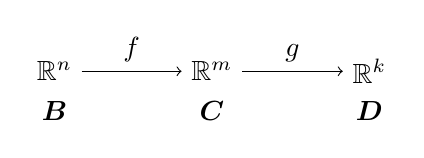
\begin{tikzpicture}
                        \node (rn) at (0, 0) {$\mathbb{R}^n$};
                        \node (rm) at (2, 0) {$\mathbb{R}^m$};
                        \node (rk) at (4, 0) {$\mathbb{R}^k$};
                        \node (b) at (0, -0.5) {$\mat{B}$};
                        \node (c) at (2, -0.5) {$\mat{C}$};
                        \node (d) at (4, -0.5) {$\mat{D}$};

                        \draw
                        (rn) edge[->] node[above]{$f$} (rm)
                        (rm) edge[->] node[above]{$g$} (rk);
                    \end{tikzpicture}
                    \\
                    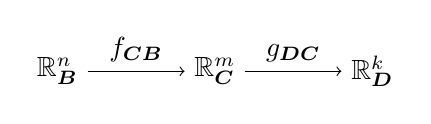
\begin{tikzpicture}
                        \node (rnb) at (0, 0) {$\mathbb{R}_{\mat{B}}^n$};
                        \node (rmc) at (2, 0) {$\mathbb{R}_{\mat{C}}^m$};
                        \node (rkd) at (4, 0) {$\mathbb{R}_{\mat{D}}^k$};

                        \draw
                        (rnb) edge[->] node[above]{$f_{\mat{C}\mat{B}}$} (rmc)
                        (rmc) edge[->] node[above]{$g_{\mat{D}\mat{C}}$} (rkd);
                    \end{tikzpicture}
                    \\
                    $g_{\mat{D}\mat{C}}f_{\mat{C}\mat{B}} = (g \circ f)_{\mat{D}\mat{B}}$
                \end{center}
                This then goes into change of basis, but see last year's \textbf{CO145}.
        \subsection*{22nd January 2020}
            \subsubsection*{Tutorial Question}
                $f : \mathbb{R}^2 \to \mathbb{R}^2$ is a linear map, and $\mat{E} = (\vec{e_1}, \vec{e_2})$ is an ordered basis.
                \begin{align*}
                    f(\vec{e_1}) & = 5\vec{e_1} - 6\vec{e_2} \\
                    f(\vec{e_2}) & = 3\vec{e_1} + \vec{e_2}
                \end{align*}
                We only care about what the linear map does to the ordered basis, as anything else can be done by linearity.
                \begin{enumerate}[(i)]
                    \itemsep0em
                    \item Find $f_{\mat{E}\mat{E}}$, the matrix representation of $f$ in $\mat{E}$ - note that this has the same input space as the output space, but it can be different.
                        \medskip

                        The first column can be done by reading the entry for for $f(\vec{e_1})$, and similarly for the second column as follows;
                        \begin{center}
                            $f_{\mat{E}\mat{E}} = \begin{bmatrix}
                                5 & 3 \\
                                -6 & 1
                            \end{bmatrix}$
                        \end{center}
                    \item If we have another ordered basis $\mat{D} = (\vec{d_1}, \vec{d_2})$, where $\vec{d_1} = \vec{e_1} - \vec{e_2}$ and $\vec{d_2} = \vec{e_1} + \vec{e_2}$, find $f_{\mat{D}\mat{D}}$.
                        \begin{center}
                            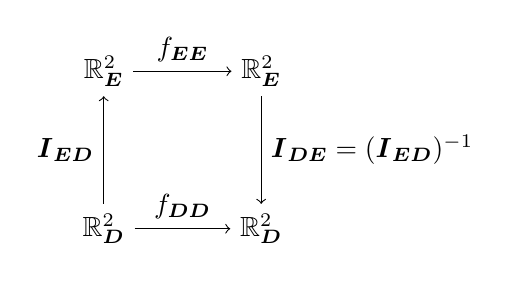
\begin{tikzpicture}
                                \node (rel) at (0, 0) {$\mathbb{R}_{\mat{E}}^2$};
                                \node (rer) at (2, 0) {$\mathbb{R}_{\mat{E}}^2$};
                                \node (rdl) at (0, -2) {$\mathbb{R}_{\mat{D}}^2$};
                                \node (rdr) at (2, -2) {$\mathbb{R}_{\mat{D}}^2$};

                                \draw
                                (rdl) edge[->] node[left]{$\mat{I}_{\mat{E}\mat{D}}$} (rel)
                                (rel) edge[->] node[above]{$f_{\mat{E}\mat{E}}$} (rer)
                                (rer) edge[->] node[right] {$\mat{I}_{\mat{D}\mat{E}} = (\mat{I}_{\mat{E}\mat{D}})^{-1}$} (rdr)
                                (rdl) edge[->] node[above]{$f_{\mat{D}\mat{D}}$} (rdr);
                            \end{tikzpicture}
                        \end{center}
                        $\mat{I}_{\mat{E}\mat{D}}$ can easily be obtained by reading the entries for $\vec{d_1}$ for the first column, and similarly for $\vec{d_2}$ in the second column;
                        \begin{align*}
                            \mat{I}_{\mat{E}\mat{D}} & = \begin{bmatrix}
                                1 & 1 \\
                                -1 & 1
                            \end{bmatrix} \\
                            \mat{I}_{\mat{D}\mat{E}} & = (\mat{I}_{\mat{E}\mat{D}})^{-1} \\
                            & = \frac{1}{2} \begin{bmatrix}
                                1 & -1 \\
                                1 & 1
                            \end{bmatrix} \\
                            f_{\mat{D}\mat{D}} & = \mat{I}_{\mat{D}\mat{E}} f_{\mat{E}\mat{E}} \mat{I}_{\mat{E}\mat{D}} \\
                            & = \frac{1}{2} \begin{bmatrix}
                                1 & -1 \\
                                1 & 1
                            \end{bmatrix} \begin{bmatrix}
                                5 & 3 \\
                                -6 & 1
                            \end{bmatrix} \begin{bmatrix}
                                1 & 1 \\
                                -1 & 1
                            \end{bmatrix} \\
                            & = \frac{1}{2} \begin{bmatrix}
                                1 & 13 \\
                                -5 & 3
                            \end{bmatrix}
                        \end{align*}
                \end{enumerate}
            \subsubsection*{Eigenvalues + Generalised Eigenvectors}
                Working with a matrix $\mat{A} \in \mathbb{C}^{m \times m}$.
                For an eigenvector $\vec{v} \in \mathbb{C}^m \setminus \{ \vec{0} \}$, and an eigenvalue $\lambda \in \mathbb{C}$, $\mat{A}\vec{v} = \lambda\vec{v} \Rightarrow (\mat{A} - \lambda\mat{I})\vec{v} = \vec{0} \Rightarrow | \mat{A} - \lambda\mat{I} | = 0 \Rightarrow P_{\mat{A}}(\lambda) = 0$ (characteristic polynomial).
                This complex polynomial will be of degree $m$, and it will have precisely $m$ roots (including multiplicity).
                Suppose $P_{\mat{A}}(\lambda) = 0$, then $(\mat{A} - \lambda\mat{I})\vec{v} = \vec{0}$ has a solution where $\vec{v} \neq \vec{0}$.
                \medskip

                Assume we have $\lambda_1, \dots, \lambda_t$ distinct eigenvalues, meaning that $P_{\mat{A}}(\lambda_i) = 0$ for $1 \leq i \leq t$.
                This means we can write the characteristic polynomial as;
                \begin{center}
                    $P_{\mat{A}}(\lambda) = (\lambda - \lambda_1)^{m_1}(\lambda - \lambda_2)^{m_2} \dots (\lambda - \lambda_t)^{m_t}$
                \end{center}
                Where $m_i$ is the \textbf{algebraic multiplicity} of $\lambda_i$. $m_i \in \mathbb{N}$, and also $1 \leq m_i \leq m$, as it must not exceed the dimension of the matrix.
                On the other hand, the \textbf{geometric multiplicity} of $\lambda_i$ is $\ell_i$, which is the \textbf{nullity} of $(\mat{A} - \lambda_i\mat{I})$.
                The nullity is the dimension of the kernel / null-space. $1 \leq \ell_i \leq m_i$, as we already have at least one non-zero solution from $(\mat{A} - \lambda_i\mat{I})\vec{v} = \vec{0}$.
                \medskip

                In the nice case, we have $\ell_i = m_i$, for $1 \leq i \leq t$, which means the matrix is diagonalisable.
                We have $m_i$ linearly independent vectors $(\vec{v_{i, 1}}, \vec{v_{i, 2}, \dots, \vec{v_{i, m_i}}})$ which satisfy
                \begin{center}
                    $\mat{A}\vec{v_{i, j}} = \lambda_i\vec{v_{i, j}}$ for $1 \leq j \leq m_i$
                \end{center}
                If we take these eigenvectors as an ordered basis;
                \begin{center}
                    $\mat{B} = [\vec{v_{1, 1}}, \vec{v_{1, 2}}, \dots, \vec{v_{1, m_1}}, \vec{v_{2, 1}}, \vec{v_{2, 2}}, \dots, \vec{v_{2, m_2}}, \dots \vec{v_{t, 1}}, \vec{v_{t, 2}}, \dots, \vec{v_{t, m_t}}]$
                \end{center}
                We also want to note that $\summation{i = 1}{t} m_i = m$, as that is the degree of the characteristic polynomial.
                Multiplying the basis by the original matrix, we get;
                \begin{center}
                    $\mat{A}\mat{B} = [\lambda_1\vec{v_{1, 1}}, \lambda_1\vec{v_{1, 2}}, \dots, \lambda_1\vec{v_{1, m_1}}, \lambda_2\vec{v_{2, 1}}, \lambda_2\vec{v_{2, 2}}, \dots, \lambda_2\vec{v_{2, m_2}}, \dots \lambda_t\vec{v_{t, 1}}, \lambda_t\vec{v_{t, 2}}, \dots, \lambda_t\vec{v_{t, m_t}}]$
                \end{center}
                Since all the columns of $\mat{B}$ are linearly independently, by our definition, the inverse $\mat{B}^{-1}$ exists.
                Therefore, we can write
                \begin{center}
                    $\mat{B}^{-1}\mat{A}\mat{B} = \begin{bmatrix}
                        \lambda_1 \\
                        & \ddots \\
                        & & \lambda_1 \\
                        & & & \lambda_2 \\
                        & & & & \ddots \\
                        & & & & & \lambda_2 \\
                        & & & & & & \ddots \\
                        & & & & & & & \lambda_t \\
                        & & & & & & & & \ddots \\
                        & & & & & & & & & \lambda_t
                    \end{bmatrix}$
                    (everything else is 0)
                \end{center}
                Which has $m_1$ instances of $\lambda_1$, followed by $m_2$ instances of $\lambda_2$, and so on, until $m_t$ instances of $\lambda_t$.
            \subsubsection*{Example for $\ell_i = m_i$}
                \begin{align*}
                    \mat{A} & = \begin{bmatrix}
                        4 & 0 & 1 \\
                        2 & 3 & 2 \\
                        1 & 0 & 4
                    \end{bmatrix} \\
                    | \mat{A} - \lambda\mat{I} | & = (\lambda - 3)^2(\lambda - 5) \\
                    \lambda_1 & = 3 & \text{two linearly independently eigenvectors} \\
                    \vec{v_{1, 1}} & = \begin{bmatrix}
                        0 \\ 1 \\ 0
                    \end{bmatrix} \\
                    \vec{v_{1, 2}} & = \begin{bmatrix}
                        -1 \\ 0 \\ 1
                    \end{bmatrix} \\
                    \lambda_2 & = 5 \\
                    \vec{v_{2, 1}} & = \begin{bmatrix}
                        1 \\ 2 \\ 1
                    \end{bmatrix} \displaybreak \\
                    \mat{B} & = \begin{bmatrix}
                        0 & -1 & 1 \\
                        1 & 0 & 2 \\
                        0 & 1 & 1
                    \end{bmatrix} \\
                    \mat{B}^{-1} & = \frac{1}{2} \begin{bmatrix}
                        -2 & 2 & -2 \\
                        -1 & 0 & 1 \\
                        1 & 0 & 1
                    \end{bmatrix} \\
                    \mat{B}^{-1}\mat{A}\mat{B} & = \begin{bmatrix}
                        3 & 0 & 0 \\
                        0 & 3 & 0 \\
                        0 & 0 & 5
                    \end{bmatrix}
                \end{align*}
            \subsubsection*{Trivial Example for $\ell_i < m_i$}
                \begin{align*}
                    \mat{A} & = \begin{bmatrix}
                        0 & 0 \\
                        0 & 1
                    \end{bmatrix} \\
                    | \mat{A} - \lambda\mat{I} | & = \lambda^2 \\
                    \lambda_1 & = 0 \\
                    \vec{v_1} & = \begin{bmatrix}
                        1 \\ 0
                    \end{bmatrix} & \text{only solution, hence } \ell_1 = 1 < 2 = m_1 \\
                    (\mat{A} - 0\mat{I}) \begin{bmatrix}
                        0 \\ 1
                    \end{bmatrix} & = \begin{bmatrix}
                        0 & 0 \\
                        0 & 1
                    \end{bmatrix} \begin{bmatrix}
                        0 \\ 1
                    \end{bmatrix} \\
                    & = \begin{bmatrix}
                        1 \\ 0
                    \end{bmatrix}
                    \intertext{although this vector is not mapped to zero, it is mapped to something that \textbf{will} be mapped to zero}
                    (\mat{A} - 0\mat{I})^2 \begin{bmatrix}
                        0 \\ 1
                    \end{bmatrix} & = (\mat{A} - 0\mat{I}) (\mat{A} - 0\mat{I}) \begin{bmatrix}
                        0 \\ 1
                    \end{bmatrix} \\
                    & = (\mat{A} - 0\mat{I}) \begin{bmatrix}
                        1 \\ 0
                    \end{bmatrix} \\
                    & = \vec{0}
                \end{align*}
                We say $\begin{bmatrix}
                    0 \\ 1
                \end{bmatrix}$ is a generalised eigenvector for $\lambda_1 = 0$.
                A vector which is not mapped by $(\mat{A} - \lambda\mat{I})$ to $\vec{0}$, but is $\vec{0}$ when iterated once more.
            \subsubsection*{Less Trivial Example}
                \begin{align*}
                    \mat{A} & = \begin{bmatrix}
                        1 & 1 & 1 \\
                        0 & 1 & 0 \\
                        0 & 0 & 1
                    \end{bmatrix} \\
                    | \mat{A} - \lambda\mat{I} | & = (1 - \lambda)^3 \\
                    \lambda_1 & = 1 & m_1 = 3 \\
                    (\mat{A} - \mat{I})\vec{x} & = \vec{0} & \Leftrightarrow \\
                    \begin{bmatrix}
                        0 & 1 & 1 \\
                        0 & 0 & 0 \\
                        0 & 0 & 0
                    \end{bmatrix} \vec{x} & = \vec{0}
                    \intertext{this has rank 1, and therefore by rank-nullity theorem (rank + nullity = 3), has 2 linearly independent solutions, therefore $\ell_1 = 2 < 3 = m_1$}
                    \vec{v_1} & = \begin{bmatrix}
                        0 \\ 1 \\ -1
                    \end{bmatrix} \displaybreak \\
                    \vec{v_2} & = \begin{bmatrix}
                        1 \\ 0 \\ 0
                    \end{bmatrix}
                    \intertext{to find the generalised eigenvector $\vec{v_3}$, we want to find some vector that is mapped by $(\mat{A} - 1 \mat{I})$ to the eigenspace, which is some linear combination of $\vec{v_1}$ and $\vec{v_2}$}
                    (\mat{A} - \mat{I}) \vec{v_3} & = \alpha_1 \vec{v_1} + \alpha_2 \vec{v_2} & \Leftrightarrow \\
                    \begin{bmatrix}
                        0 & 1 & 1 \\
                        0 & 0 & 0 \\
                        0 & 0 & 0
                    \end{bmatrix} \begin{bmatrix}
                        x_1 \\ x_2 \\ x_3
                    \end{bmatrix} & = \begin{bmatrix}
                        0 \\ \alpha_1 \\ -\alpha_1
                    \end{bmatrix} + \begin{bmatrix}
                        \alpha_2 \\ 0 \\ 0
                    \end{bmatrix} \\
                    & = \begin{bmatrix}
                        x_2 + x_3 \\ 0 \\ 0
                    \end{bmatrix} & \Leftrightarrow \\
                    \alpha_1 & = 0 \\
                    x_2 + x_3 & = \alpha_2 & \text{let } x_2 = 0 \Rightarrow x_3 = \alpha_2 = 1 \\
                    \vec{v_3} & = \begin{bmatrix}
                        0 \\ 0 \\ 1
                    \end{bmatrix} \\
                    \mat{B} & = [\vec{v_1}, \vec{v_2}, \vec{v_3}] \\
                    & = \begin{bmatrix}
                        0 & 1 & 0 \\
                        1 & 0 & 0 \\
                        -1 & 0 & 1
                    \end{bmatrix} \\
                    \mat{B}^{-1}\mat{A}\mat{B} & = \begin{bmatrix}
                        1 & 0 & 0 \\
                        0 & 1 & 1 \\
                        0 & 0 & 1
                    \end{bmatrix} & \text{the extra 1 is from $\vec{v_2}$?}
                \end{align*}
                This is in Jordan Normal Form.
                For some $\lambda_i$ eigenvalue, and $\ell_i \leq m_i$, the sum of the sizes of the blocks is $m_i$, and the number of blocks is $\ell_i$.
                If $\lambda_i$ is an eigenvalue of $\mat{A}$ with algebraic multiplicity $m_i$, then the nullity of $(\mat{A} - \lambda_i \mat{I})^{m_i} = m_i$.
                \medskip

                \textbf{Definition}: $\vec{v} \in \mathbb{R}^m$ is a generalised eigenvector for $\lambda_i$ if $(\mat{A} - \lambda_i \mat{I})^{m_i} \vec{v} = \vec{0}$.
                The maximum iterations is $m_i$, but can be less.
        \subsection*{23rd January 2020}
            In general;
            \begin{itemize}
                \itemsep0em
                \item $\forall j\ [\ell_j = m_j] \Rightarrow \mat{A}$ is diagonalisable
                \item $\exists j\ [\ell_j < m_j] \Rightarrow \mat{A}$ is diagonalisable or \textbf{almost} diagonalisable
            \end{itemize}
            The following is a very poor explanation of what the form looks like, because I don't know how to draw blocks in \LaTeX.
            See Panopto at timestamp 13:17 for a proper drawing.
            \begin{align*}
                \mat{A} & = \begin{bmatrix}
                    \mat{B_{\lambda_1}} \\
                    & \ddots \\
                    & & \mat{B_{\lambda_t}}
                \end{bmatrix} \\
                \mat{B_j} & = \begin{bmatrix}
                    \mat{J_j} \\
                    & \ddots \\
                    & & \mat{J_j}
                \end{bmatrix} & \text{all $\mat{J_j}$ can be of different sizes, $\mat{B_j} \in \mathbb{R}^{m_j \times m_j}$} \displaybreak \\
                \mat{J_i} & = \begin{bmatrix}
                    \lambda_i & 1 \\
                    & \lambda_i & \ddots \\
                    & & \ddots & 1 \\
                    & & & \lambda_i
                \end{bmatrix}
            \end{align*}
            \subsubsection*{Spectral Decomposition of Symmetric Matrices}
                In almost all areas of computer science, symmetric matrices are the dominant paradigm.
                All the eigenvalues of real symmetric matrices are real, and are always diagonalisable.
                A symmetric matrix is always a square matrix $\mat{A} \in \mathbb{R}^{n \times n}$, which also satisfies $\mat{A}^\top = \mat{A}$, meaning it is symmetric along the diagonal (the elements above the diagonal determine the elements below, and vice versa).
                We are to prove the following properties;
                \begin{enumerate}[(i)]
                    \itemsep0em
                    \item All eigenvalues of $\mat{A}$ are real.
                        \medskip

                        First assume that $\vec{v} \in \mathbb{C}^n$, as we don't yet know that it is real, therefore we can have the case $\lambda \in \mathbb{C}$.
                        \begin{align*}
                            \mat{A}\vec{v} & = \lambda\vec{v} & \Rightarrow \\
                            \vec{v}^{*^\top}\mat{A}\vec{v} & = \lambda \vec{v}^{*^\top}\vec{v} \\
                            & = \lambda || \vec{v} ||^2 & (1) \\
                            \vec{v}^{*^\top}\mat{A}\vec{v} & = \left(\vec{v}^{*^\top}\mat{A}\right)\vec{v} \\
                            & = \left((\mat{A}\vec{v})^\top\right)^* \vec{v}
                            \intertext{briefly proving the above;}
                            \left((\mat{A}\vec{v})^\top\right)^* & = \left(\vec{v}^\top\mat{A}^\top\right)^* & \text{taking the transpose inside the bracket} \\
                            & = \left(\vec{v}^\top\right)^* \mat{A}^* & \text{taking the conjugate inside and $\mat{A}^\top = \mat{A}$} \\
                            & = \left(\vec{v}^\top\right)^* \mat{A} & \text{$\mat{A}$ is real valued matrix}
                            \intertext{continuing on;}
                            & = \left((\lambda\vec{v})^\top\right)^* \vec{v} & \text{$\vec{v}$ is an eigenvector} \\
                            & = \lambda^* \left(\vec{v}^\top\right)^* \vec{v} & \text{transposing a scalar does nothing} \\
                            & = \lambda^* || \vec{v} ||^2 & (2)
                        \end{align*}
                        By comparing results, $(1) = (2)$, hence $\lambda^* = \lambda$ (dividing through by $|| \vec{v} ||^2$ is allowed, since we know it is non-zero by properties of vector norms, and $\vec{v} \neq \vec{0}$ by properties of eigenvectors).
                        As the complex conjugate of $\lambda$ is the same as $\lambda$, we can conclude that $\lambda \in \mathbb{R}$.
                    \item Eigenvectors corresponding to different eigenvalues of $\mat{A}$ are perpendicular.
                        \medskip

                        Note that with the above result, we know that $\vec{v} \in \mathbb{R}^n$, as there is no possible way to obtain complex values with a real valued matrix and a real valued eigenvalue.
                        \begin{align*}
                            \mat{A}\vec{v_1} & = \lambda_1 \vec{v_1} \\
                            \mat{A}\vec{v_2} & = \lambda_2 \vec{v_2} \\
                            \lambda_1 & \neq \lambda_2 \\
                            \vec{v_2}^\top\mat{A}\vec{v_1} & = \lambda_1 \vec{v_2}^\top \vec{v_1} \\
                            & = \lambda_1 (\vec{v_1} \cdot \vec{v_2}) & (1) \\
                            \vec{v_2}^\top\mat{A}\vec{v_1} & = \left(\vec{v_2}^\top\mat{A}\right)\vec{v_1} \\
                            & = (\mat{A}\vec{v_2})^\top\vec{v_1} & \text{adding a transpose and $\mat{A}^\top = \mat{A}$} \\
                            & = \lambda_2 \vec{v_2}^\top \vec{v_1} & \text{$\vec{v_2}$ is an eigenvector} \\
                            & = \lambda_2 (\vec{v_1} \cdot \vec{v_2}) & (2)
                        \end{align*}
                        Similarly, comparing results (1) and (2), we get
                        \begin{align*}
                            \lambda_1 (\vec{v_1} \cdot \vec{v_2}) & = \lambda_2 (\vec{v_1} \cdot \vec{v_2}) & \Leftrightarrow \\
                            \lambda_1 (\vec{v_1} \cdot \vec{v_2}) - \lambda_2 (\vec{v_1} \cdot \vec{v_2}) & = 0 \\
                            (\lambda_1 - \lambda_2)(\vec{v_1} \cdot \vec{v_2}) & = 0 & \Leftrightarrow \\
                            \lambda_1 & = \lambda_2 \\
                            \text{or } \vec{v_1} \cdot \vec{v_2} & = 0
                        \end{align*}
                        The former is not possible due to the condition that they are different eigenvalues, therefore $\vec{v_1} \cdot \vec{v_2} = 0$.
                        As neither are the zero vector, by definition of eigenvectors, $\cos \theta = 0$, therefore they are perpendicular.
                    \item (Tutorial 3) If $\lambda_j$ is an eigenvalue of $\mat{A}$ then $\ell_j = m_j$, therefore $\mat{A}$ is diagonalisable.
                        \medskip

                        Come back to this in two weeks?
                \end{enumerate}
                To conclude, we get all the eigenvectors and we normalise them (divide by the $\ell_2$-norm), and we can assume they are pairwise orthogonal.
                There is an orthonormal basis for $\mathbb{R}^n$ consisting of eigenvectors of $\mathbb{A}$; $(\vec{v_1}, \dots, \vec{v_n})$, where $\vec{v_j} \in \mathbb{R}^n$.
                This has the following properties;
                \begin{itemize}
                    \itemsep0em
                    \item $\mat{A}\vec{v_j} = \lambda_j \vec{v_j}$
                    \item $\vec{v_i} \bot \vec{v_j}$, when $i \neq j$ \hfill perpendicular
                    \item $|| \vec{v_i} || = 1$ for $i = 1, \dots, n$
                \end{itemize}
            \subsubsection*{Examples}
                For an example in $\mathbb{R}^{2 \times 2}$;
                \begin{align*}
                    \mat{A} & = \begin{bmatrix}
                        1 & 2 \\
                        2 & 1
                    \end{bmatrix} \\
                    | \mat{A} - \lambda\mat{I} | & = (1 - \lambda)^2 - 4 \\
                    \lambda_1 & = 3 \\
                    \lambda_2 & = -1 \\
                    \vec{v_1} & = \frac{1}{\sqrt{2}} \begin{bmatrix}
                        1 \\ 1
                    \end{bmatrix} & \text{normalise straight away} \\
                    \vec{v_2} & = \frac{1}{\sqrt{2}} \begin{bmatrix}
                        1 \\ -1
                    \end{bmatrix} \\
                    \mat{V} & = [\vec{v_1}, \vec{v_2}] & \text{orthonormal basis of } \mathbb{R}^2 \\
                    & = \frac{1}{\sqrt{2}} \begin{bmatrix}
                        1 & 1 \\
                        1 & -1
                    \end{bmatrix} \\
                    \mat{A}\mat{V} & = [\mat{A}\vec{v_1}, \mat{A}\vec{v_2}] \\
                    & = [3 \vec{v_1}, - \vec{v_2}]
                    \intertext{For a symmetric matrix, if we have a matrix $\mat{V}$ representing the orthonormal basis of the eigenvectors, $\mat{V}^{-1} = \mat{V}^\top$}
                    \mat{V}^{-1}\mat{A}\mat{V} & = \mat{V}^\top\mat{A}\mat{V} \\
                    & = \mat{V}^\top [3 \vec{v_1}, - \vec{v_2}] \\
                    & = \begin{bmatrix}
                        \vec{v_1}^\top \\
                        \vec{v_2}^\top
                    \end{bmatrix} [3 \vec{v_1}, - \vec{v_2}] \\
                    & = \begin{bmatrix}
                        3 & 0 \\
                        0 & -1
                    \end{bmatrix} & \text{dot product with unit length ($\vec{v_1} \bot \vec{v_2}$)}
                \end{align*}
                For an example in $\mathbb{R}^{3 \times 3}$;
                \begin{align*}
                    \mat{A} & = \begin{bmatrix}
                        1 & 1 & 3 \\
                        1 & 3 & 1 \\
                        3 & 1 & 1
                    \end{bmatrix}
                    \intertext{now he just shows some intuition on getting an eigenvalue?}
                    | \mat{A} - \lambda\mat{I} | & = \begin{vmatrix}
                        1 - \lambda & 1 & 3 \\
                        1 & 3 - \lambda & 1 \\
                        3 & 1 & 1 - \lambda
                    \end{vmatrix} \\
                    & = \begin{vmatrix}
                        5 - \lambda & 1 & 3 \\
                        5 - \lambda & 3 - \lambda & 1 \\
                        5 - \lambda & 1 & 1 - \lambda
                    \end{vmatrix} & \vec{c_1}^\prime = \vec{c_1} + \vec{c_2} + \vec{c_3} \\
                    & = 0 \\
                    \lambda_1 & = 5 \\
                    \text{trace}(\mat{A}) & = \lambda_1 + \lambda_2 + \lambda_3 \\
                    & = 5 & \Rightarrow \\
                    \lambda_2 + \lambda_3 & = 0 \\
                    | \mat{A} | & = \lambda_1 \lambda_2 \lambda_3 \\
                    & = -20 & \Rightarrow \\
                    \lambda_2 \lambda_3 & = -4 \\
                    \lambda_2 & = 2 \\
                    \lambda_3 & = -2 \\
                    \vec{v_1} & = \frac{1}{\sqrt{3}} \begin{bmatrix}
                        1 \\ 1 \\ 1
                    \end{bmatrix} \\
                    \vec{v_2} & = \frac{1}{\sqrt{6}} \begin{bmatrix}
                        1 \\ -2 \\ 1
                    \end{bmatrix} \\
                    \vec{v_3} & = \frac{1}{\sqrt{2}} \begin{bmatrix}
                        1 \\ 0 \\ 1
                    \end{bmatrix} \\
                    \mat{V} & = [\vec{v_1}, \vec{v_2}, \vec{v_3}] \\
                    \mat{V}^{-1} & = \mat{V}^\top \\
                    \mat{V}^{-1}\mat{A}\mat{V} & = \mat{V}^\top\mat{A}\mat{V} \\
                    & = \begin{bmatrix}
                        5 & 0 & 0 \\
                        0 & 2 & 0 \\
                        0 & 0 & -2
                    \end{bmatrix} & \text{spectral decomposition of a symmetric matrix}
                \end{align*}
            \subsubsection*{Proof of $\mat{V}^{-1} = \mat{V}^\top$}
                We define $\mat{B} \in \mathbb{R}^{n \times n}$ as an \textbf{orthogonal matrix} if all columns $\vec{b_j}$ for $1 \leq j \leq n$ form an orthonormal basis of $\mathbb{R}^n$, such that the two properties hold;
                \begin{itemize}
                    \itemsep0em
                    \item $\vec{b_j} \cdot \vec{b_i} = 0$ when $i \neq j$
                    \item $\vec{b_j} \cdot \vec{b_j} = 1$
                \end{itemize}
                We want to prove that $\mat{B}^{-1} = \mat{B}^\top$:
                \begin{align*}
                    \mat{B} & = [\vec{b_1}, \dots, \vec{b_n}] \\
                    \mat{B}^\top & = \begin{bmatrix}
                        \vec{b_1}^\top \\
                        \vdots \\
                        \vec{b_n}^\top
                    \end{bmatrix} \\
                    \mat{B}^\top\mat{B} & = \begin{bmatrix}
                        \vec{b_1}^\top \\
                        \vdots \\
                        \vec{b_n}^\top
                    \end{bmatrix} [\vec{b_1}, \dots, \vec{b_n}] \\
                    & = \begin{bmatrix}
                        1 & 0 & \cdots & 0 \\
                        0 & 1 & \ddots & \vdots \\
                        \vdots & \ddots & \ddots & 0 \\
                        0 & \cdots & 0 & 1
                    \end{bmatrix} \\
                    & = \mat{I}_n
                \end{align*}
            \subsubsection*{Preservation of Length}
                The length of a vector $\vec{x}$ is preserved under orthogonal transformation;
                \begin{align*}
                    (\mat{V}\vec{x}) \cdot (\mat{V}\vec{x}) & = (\mat{V}\vec{x})^\top (\mat{V}\vec{x}) \\
                    & = \vec{x}^\top \mat{V}^\top \mat{V} \vec{x} \\
                    & = \vec{x}^\top \mat{V}^{-1} \mat{V} \vec{x} \\
                    & = \vec{x}^\top \vec{x} \\
                    & = \vec{x} \cdot \vec{x}
                \end{align*}
            \subsubsection*{Geometric Intuition}
                Take a real symmetric matrix $\mat{A} \in \mathbb{R}^{n \times n}$, such that $\mat{A}^\top = \mat{A}$.
                Assume we have processed it to get the eigenvalues $\lambda_1, \dots, \lambda_n$, such that $\mat{V}^\top\mat{A}\mat{V} = \text{diag}(\lambda_1, \dots, \lambda_n)$, and $\mat{V}$ is an orthonormal matrix formed of the eigenvectors.
                \medskip

                Take a vector $\vec{x}$ from the input space, to $\mat{A}\vec{x}$ in the output space, mapped by $\mat{A}$;
                \begin{center}
                    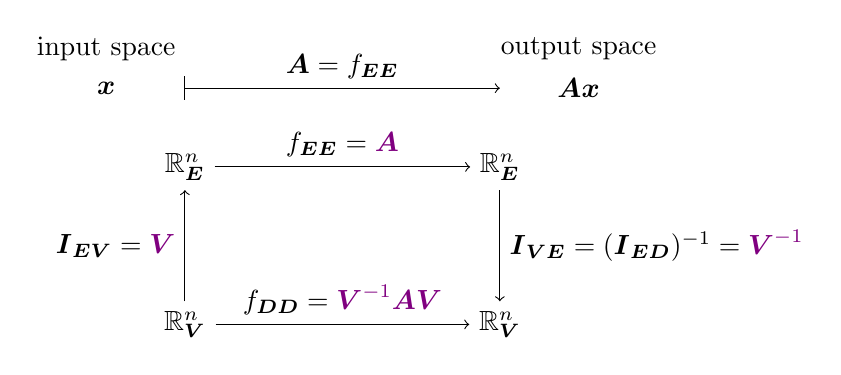
\begin{tikzpicture}
                        \node at (0, 0.5) {input space};
                        \node at (6, 0.5) {output space};

                        \node (x) at (0, 0) {$\vec{x}$};
                        \node (ax) at (6, 0) {$\mat{A}\vec{x}$};

                        \draw
                        (1, 0.15) -- (1, -0.15)
                        (1, 0) edge[->] node[above] {$\mat{A} = f_{\mat{E}\mat{E}}$} (5, 0);

                        \node (rel) at (1, -1) {$\mathbb{R}_{\mat{E}}^n$};
                        \node (rer) at (5, -1) {$\mathbb{R}_{\mat{E}}^n$};
                        \node (rvl) at (1, -3) {$\mathbb{R}_{\mat{V}}^n$};
                        \node (rvr) at (5, -3) {$\mathbb{R}_{\mat{V}}^n$};

                        \draw
                        (rvl) edge[->] node[left]{$\mat{I}_{\mat{E}\mat{V}} = \violet{\mat{V}}$} (rel)
                        (rel) edge[->] node[above]{$f_{\mat{E}\mat{E}} = \violet{\mat{A}}$} (rer)
                        (rer) edge[->] node[right] {$\mat{I}_{\mat{V}\mat{E}} = (\mat{I}_{\mat{E}\mat{D}})^{-1} = \violet{\mat{V}^{-1}}$} (rvr)
                        (rvl) edge[->] node[above]{$f_{\mat{D}\mat{D}} = \violet{\mat{V}^{-1}\mat{A}\mat{V}}$} (rvr);
                    \end{tikzpicture}
                \end{center}
                Consider a unit sphere, created by $|| \vec{x} || = 1$, where $\vec{x} \in \mathbb{R}^3$.
                The transformations $\mat{V}^{-1} = \mat{V}^\top$ and $\mat{V}$ are rotations as they preserve length.
                Take a point $\vec{x}$ on the surface of this unit sphere, applying $\mat{V}^{-1}$ to it simply rotates it to another point on the surface of the sphere (going from $\mathbb{R}_{\mat{E}}^3$ to $\mathbb{R}_{\mat{V}}^3$) in the input space.
                Let this point have coordinates $\vec{u}$ with respect to $\mat{V}$.
                Under the diagonal map $\text{diag}(\lambda_1, \dots, \lambda_n)$, we get the following;
                \begin{center}
                    $u_1 \vec{v_1} + \dots + u_n \vec{v_n} \mapsto \lambda_1 u_1 \vec{v_1} + \dots + \lambda_n u_n \vec{v_n}$
                \end{center}
                As $\vec{u}$ is on the sphere, we can say;
                \begin{center}
                    $|| \vec{u} ||_2^2 = u_1^1 + \dots + u_n^2 = 1$
                \end{center}
                Therefore, the mapped point $\vec{y}$ can be written as $\begin{bmatrix}
                    \lambda_1 u_1 \\ \vdots \\ \lambda_n u_n
                \end{bmatrix}$, satisfying (in three dimensions);
                $$\frac{y_1^2}{\lambda_1^2} + \frac{y_2^2}{\lambda_2^2} + \frac{y_3^2}{\lambda_3^2} = 1$$
                This gives a locus of an ellipsoid.
            \subsubsection*{Rank-Nullity Theorem}
                Take a matrix $\mat{A} \in \mathbb{R}^{m \times n}$.
                \begin{align*}
                    \text{Im}(\mat{A}) \subseteq \mathbb{R}^m & = \{ \mat{A}\vec{x} : \vec{x} \in \mathbb{R}^n\} \\
                    \text{dim}(\text{Im}(\mat{A})) & = \text{column rank of } \mat{A} \\
                    \text{Null}(\mat{A}) \subseteq \mathbb{R}^n & = \{ \vec{v} : \mat{A}\vec{v} = \vec{0} \} & \text{same as kernel} \\
                    \text{rk}(\text{column space}) & = \text{rk}(\text{row space}) \\
                    \text{row space } \mat{A} & = \text{column space } \mat{A}^\top
                \end{align*}
                For elementary row operations, we have the following property;
                \begin{enumerate}[(I)]
                    \itemsep0em
                    \item they are invertible.
                        \medskip

                        If there is one of the three elementary row operations $R$ that takes $\mat{A} \leadsto \mat{B}$, then $\exists R^{-1}$ that takes $\mat{B} \leadsto \mat{A}$.
                        \smallskip

                        If $\mat{A} \leadsto \mat{B}$, then $\mat{B} = \mat{M_R}\mat{A}$.
                        We obtain $\mat{M_R}$ by applying $R$ to $\mat{I}_m$, such that $\mat{I}_m \leadsto \mat{M_R}$.
                \end{enumerate}
                A reduction to row echelon form can be written as follows (with $-$ as a pivot, and $\times$ being any number);
                $$\mat{A} \overset{R_1}{\leadsto} \cdots \overset{R_t}{\leadsto} \mat{C} = \begin{bmatrix}
                    - & \times & \times & \times & \times & \times \\
                    0 & - & \times & \times & \times & \times \\
                    0 & 0 & 0 & - & \times & \times \\
                    0 & 0 & 0 & 0 & - & \times \\
                    0 & 0 & 0 & 0 & 0 & - \\
                    \hline
                    0 & 0 & 0 & 0 & 0 & 0
                \end{bmatrix}$$
                In general it creates a staircase of the pivots, and everything below it is 0.
                Note that the example above is just a random example, as long as the general structure remains, it's fine.
                \medskip

                An ERO doesn't change the row space, as it is operating on the rows.
                Swapping rows, multiplying by a non-zero number, and adding rows will not change anything.
                The claim is that while the column space can change, the rank of the column space doesn't change.
                \begin{align*}
                    \mat{A} & = [\vec{a_1}, \dots, \vec{a_n}] \\
                    \mat{A} \overset{R}{\leadsto} \mat{M_R}\mat{A} & = [\mat{M_R}\vec{a_1}, \dots, \mat{M_R}\vec{a_n}] \\
                    \mat{M_{R^{-1}}} & = (\mat{M_R})^{-1} & \text{therefore $\mat{M_R}$ is invertible}
                    \intertext{taking some linear combination of the vectors in $\mat{A}$}
                    \lambda_1 \vec{a_{i_1}} + \dots + \lambda_1 \vec{a_{i_t}} & = 0 & \Leftrightarrow \\
                    \mat{M_R}(\lambda_1 \vec{a_{i_1}} + \dots + \lambda_1 \vec{a_{i_t}}) & = 0
                \end{align*}
                This is due to the fact that multiplying a set of linearly independent vectors by an invertible matrix preserves independence.
                From this it follows that the dimension of the columns of $\mat{A}$ is equal to the dimension of the columns of $\mat{M_R}\mat{A}$, since $\mat{M_R}$ is invertible.
                Therefore neither the row rank nor the column rank changes.
                \medskip

                Since $\mat{C}$ is in REF, the row rank is equal to the column rank, which is equal to the number of pivots, let it be $r$, then $\text{rk}(\mat{A}) = r$.
        \subsection*{29th January 2020}
            \subsubsection*{Properties of Symmetric Matrices}
                Take $\mat{A} \in \mathbb{R}^{n \times n}$, such that $\mat{A}^\top = \mat{A}$.
                \medskip

                All eigenvalues of $\mat{A}$ are positive \violet{(non-negative)} iff $\forall \vec{x} \in \mathbb{R}^{n} \setminus \{ \vec{0} \}\ [\vec{x}^\top\mat{A}\vec{x} > 0 \violet{(\geq 0)}]$.
                $\vec{x}^\top\mat{A}\vec{x}$ is called a quadratic form.
                For example;
                \begin{align*}
                    \mat{A} & = \begin{bmatrix}
                        a & b \\
                        b & c
                    \end{bmatrix} \\
                    \vec{x} & = \begin{bmatrix}
                        x_1 \\ x_2
                    \end{bmatrix} \\
                    \vec{x}^\top\mat{A}\vec{x} & = \begin{bmatrix}
                        x_1 & x_2
                    \end{bmatrix} \begin{bmatrix}
                        a & b \\
                        b & c
                    \end{bmatrix} \begin{bmatrix}
                        x_1 \\ x_2
                    \end{bmatrix} \\
                    & = ax_1^2 + 2bx_1x_2 + cx_2^2 \\
                    & = k \\
                    \text{assume } x_2 & \neq 0 \\
                    \frac{\vec{x}^\top\mat{A}\vec{x}}{x_2^2} & = ay^2 + 2b^y + c & \text{where } y = \frac{x_1}{x_2} \\
                    & > 0 & \text{focusing on the positive case}
                \end{align*}
                If $\vec{x}^\top\mat{A}\vec{x} > 0$, then we have an ellipse, with slanted major / minor axes.
                This uses a similar result to the result with the sphere's orthonormal basis being formed from the eigenvectors.
                \medskip

                Considering this algebraically, if the quadratic in $y$ is always greater than 0, then it must have no roots, hence the discriminant must be negative.
                Therefore we have the case where $(2b)^2 - 4ac < 0$, so $b^2 - ac < 0$, and $a > 0$.
                \medskip

                Using the properties of the trace and the determinant, we can state the following;
                \begin{align*}
                    \lambda_1 + \lambda_2 & = a + c \\
                    \lambda_1 \lambda_2 & = ac - b^2
                \end{align*}
                We want both $ac - b^2$ and $a + b$ to be positive.
                The former is shown with the result for the discriminant, as if $b^2 - ac$ is negative, then $ac - b^2$ must be positive.
                The latter then follows as $c$ is positive only if $a$ is positive (due to $ac > b^2 \geq 0$), which we have previously.
                This shows it holds for the simple case.
                \medskip

                The proof for any $n > 1$ is as follows;
                \begin{align*}
                    \mat{S} & = \text{diag}(\lambda_1, \dots, \lambda_n) \\
                    & = \mat{V}^\top\mat{A}\mat{V} & \Rightarrow \\
                    \mat{A} & = \mat{V}\mat{S}\mat{V}^\top & \Rightarrow \\
                    \vec{x}^\top\mat{A}\vec{x} & = \vec{x}^\top\mat{V}\mat{S}\mat{V}^\top\vec{x} \\
                    & = \vec{z}^\top\mat{S}\vec{z} & \text{where } \vec{z} = \mat{V}^\top\vec{x} \text{(which preserves $\ell_2$-norm)} \\
                    & = \summation{i = 1}{n} \lambda_i z_i^2
                \end{align*}
                To say $\vec{x}^\top\mat{A}\vec{x}$ is positive for any non-zero $\vec{x}$ is to say that $\summation{i = 1}{n} \lambda_i z_i^2$ is positive for any non-zero $\vec{v}$.
                \smallskip

                Then obviously all the eigenvalues ($\lambda_i$) must be positive iff $\summation{i = 1}{n} \lambda_i z_i^2$ is positive.
            \subsubsection*{Singular Value Decomposition (SVD)}
                This works for a \textbf{general} matrix (not necessarily square).
                Take any matrix $\mathbb{R}^{m \times n}$.
                \begin{center}
                    $\exists \mat{V} \in \mathbb{R}^{n \times n}, \mat{U} \in \mathbb{R}^{m \times m}, \sigma_1 \geq \sigma_2 \geq \dots \geq \sigma_r > \sigma_{r + 1} = \dots = \sigma_p = 0$
                \end{center}
                Where $\mat{V}$, $\mat{U}$ are orthogonal matrices, $p = \min (m, n)$, and $r = \text{rk}(\mat{A})$.
                We have a finitely decreasing sequence of $\sigma$.
                This allows us to write the following (assuming $n \leq m$);
                \begin{center}
                    $\mat{A} = \mat{U}\mat{S}\mat{V}^\top$, where $\mat{S} = \begin{bmatrix}
                        \sigma_1 \\
                        & \sigma_2 \\
                        & & \ddots \\
                        & & & \sigma_r \\
                        & & & & 0 \\
                        & & & & & \ddots \\
                        & & & & & & 0 \\
                        \hline
                        0 & & & \dots & & & 0 \\
                        \vdots & & & \ddots & & & \vdots \\
                        0 & & & \dots & & & 0 \\
                    \end{bmatrix}$
                \end{center}
                This is the singular value decomposition of $\mat{A}$, and $\sigma_1, \dots, \sigma_r$ are the singular values of $\mat{A}$.
                $\sigma_1$ is the largest singular value of $\mat{A}$, which is the $\ell_2$ matrix norm of $\mat{A}$ ($|| \mat{A} ||_2$).
                The geometric intuition of this, in two dimensions, is as follows;
                \begin{center}
                    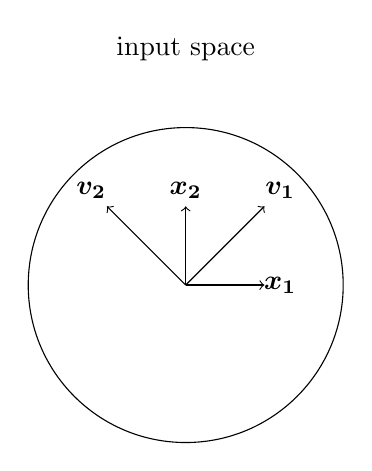
\begin{tikzpicture}
                        \node at (0, 3) {input space};

                        \node at (1.2, 0) {$\vec{x_1}$};
                        \node at (0, 1.2) {$\vec{x_2}$};
                        \node at (1.2, 1.2) {$\vec{v_1}$};
                        \node at (-1.2, 1.2) {$\vec{v_2}$};

                        \draw
                        (0, 0) edge[->] (1, 0)
                        (0, 0) edge[->] (0, 1)
                        (0, 0) edge[->] (1, 1)
                        (0, 0) edge[->] (-1, 1);
                        \draw (0, 0) circle (2);
                    \end{tikzpicture}
                    \ \ \ \ \
                    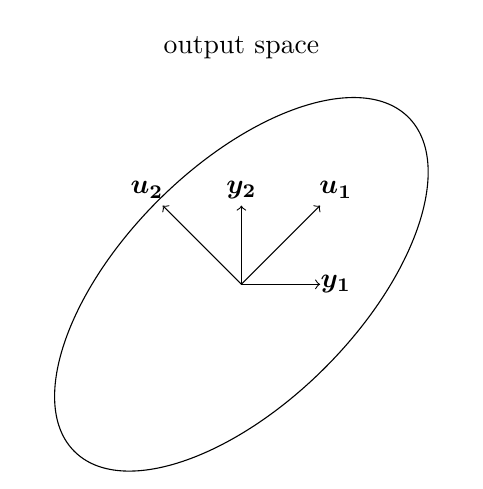
\begin{tikzpicture}
                        \node at (0, 3) {output space};

                        \node at (1.2, 0) {$\vec{y_1}$};
                        \node at (0, 1.2) {$\vec{y_2}$};
                        \node at (1.2, 1.2) {$\vec{u_1}$};
                        \node at (-1.2, 1.2) {$\vec{u_2}$};

                        \draw
                        (0, 0) edge[->] (1, 0)
                        (0, 0) edge[->] (0, 1)
                        (0, 0) edge[->] (1, 1)
                        (0, 0) edge[->] (-1, 1);
                        \draw[rotate=-45] (0, 0) circle (1.5 and 3);
                    \end{tikzpicture}
                \end{center}
                Starting with our coordinates in the basis $(\vec{x_1}, \vec{x_2})$, the matrix $\mat{V}^\top$ performs a rotation to the new basis $(\vec{v_1}, \vec{v_2})$.

                Take some point $\vec{x}$ on the unit circle with coordinates $\begin{bmatrix}
                    x_1 \\ x_2
                \end{bmatrix}$, we obtain the new coordinates $\begin{bmatrix}
                    v_1 \\ v_2
                \end{bmatrix} = \mat{V}^\top\vec{x}$.

                We still maintain $|| \vec{x} || = 1$ and $|| \vec{v} || = 1$.

                We're now in the basis of $(\vec{u_1}, \vec{u_2})$.
                We can say that $u_1 = \sigma_1 v_1$, $u_2 = \sigma_2 v_2$ (and so on, for higher dimensions).
                This implies the following result;
                $$\frac{u_1^2}{\sigma_1^2} + \frac{u_2^2}{\sigma_2^2} = v_1^2 + v_2^2 = 1$$
                Hence we obtain an ellipse.
            \subsubsection*{Example}
                \begin{align*}
                    \mat{A} \in \mathbb{R}^{3 \times 2} & = \begin{bmatrix}
                        1 & -1 \\
                        -1 & 1 \\
                        1 & -1
                    \end{bmatrix} \\
                    \text{rk}(\mat{A}) & = 1 \\
                    \mat{A} & = \mat{U}\mat{S}\mat{V}^\top \\
                    \mat{S} \in \mathbb{R}^{3 \times 2} & = \text{diag}(\sigma_1, \sigma_2, \dots) \\
                    \mat{A}^\top & = \left(\mat{V}^\top\right)^\top\mat{S}^\top\mat{U}^\top \\
                    & = \mat{V}\mat{S}^\top\mat{U}^\top \\
                    \mat{A}^\top\mat{A} & = \mat{V}\mat{S}^\top\mat{U}^\top\mat{U}\mat{S}\mat{V}^\top \\
                    & = \mat{V}\mat{S}^\top\mat{S}\mat{V}^\top & \mat{U} \text{ is an orthogonal matrix}
                    \intertext{brief note on $\mat{S}^\top\mat{S} \in \mathbb{R}^{2 \times 2}$}
                    \mat{S}^\top\mat{S} & = \text{diag}(\sigma_1, \sigma_2, \dots)\ \text{diag}(\sigma_1, \sigma_2, \dots) \\
                    & = \text{diag}(\sigma_1^2, \sigma_2^2, \dots)
                    \intertext{brief proof for symmetry of $\mat{A}^\top\mat{A}$}
                    \left(\mat{A}^\top\mat{A}\right)^\top & = \mat{A}^\top\left(\mat{A}^\top\right)^\top \\
                    & = \mat{A}^\top\mat{A}
                    \intertext{$\mat{A}^\top\mat{A}$ is also positive semi-definite, meaning all its eigenvalues are non-negative ($\geq 0$) since}
                    \vec{x}^\top\mat{A}^\top\mat{A}\vec{x} & = (\mat{A}\vec{x})^\top(\mat{A}\vec{x}) \\
                    & \geq 0
                \end{align*}
                In this form, all we have to do is to find the spectral decomposition for $\mat{A}^\top\mat{A}$, since we have a symmetric matrix.
                \begin{align*}
                    \mat{A}^\top\mat{A} & = \begin{bmatrix}
                        3 & -3 \\
                        -3 & 3
                    \end{bmatrix} \\
                    | \mat{A}^\top\mat{A} - \lambda\mat{I} | & = (3 - \lambda)^2 - 9 \\
                    \lambda_1 & = 6 & \Rightarrow \\
                    \sigma_1 & = \sqrt{6} \\
                    \vec{v_1} & = \frac{1}{\sqrt{2}} \begin{bmatrix}
                        1 \\ -1
                    \end{bmatrix} \\
                    \lambda_2 & = 0 & \Rightarrow \\
                    \sigma_2 & = 0 \\
                    \vec{v_2} & = \frac{1}{\sqrt{2}} \begin{bmatrix}
                        1 \\ 1
                    \end{bmatrix} \\
                    \mat{V} & = [\vec{v_1}, \vec{v_2}] \\
                    & = \frac{1}{\sqrt{2}} \begin{bmatrix}
                        1 & 1 \\
                        -1 & 1
                    \end{bmatrix} \\
                    \mat{A}\mat{V} & = \mat{U}\mat{S} & \Rightarrow \\
                    [\mat{A}\vec{v_1}, \mat{A}\vec{v_2}] & = \mat{U} \begin{bmatrix}
                        \sqrt{6} & 0 \\
                        0 & 0 \\
                        0 & 0
                    \end{bmatrix} \\
                    & = [\sqrt{6} \vec{u_1}, \vec{0}] & \Rightarrow \displaybreak \\
                    \vec{u_1} & = \frac{1}{\sqrt{6}}\mat{A}\vec{v_1} \\
                    & = \frac{1}{\sqrt{3}} \begin{bmatrix}
                        1 \\ -1 \\ 1
                    \end{bmatrix} \\
                    \vec{u_2} & = \frac{1}{\sqrt{2}} \begin{bmatrix}
                        1 \\ 1 
                    \end{bmatrix} & \text{unit vector orthogonal to $\vec{u_1}$} \\
                    \vec{u_3} & = \vec{u_1} \times \vec{u_2} \\
                    & = \frac{1}{\sqrt{6}} \begin{bmatrix}
                        1 \\ -1 \\ -2
                    \end{bmatrix} \\
                    \mat{A} & = [\vec{u_1}, \vec{u_2}, \vec{u_3}] \begin{bmatrix}
                        \sqrt{6} & 0 \\
                        0 & 0 \\
                        0 & 0
                    \end{bmatrix} [\vec{v_1}, \vec{v_2}]
                \end{align*}
        \subsection*{30th January 2020}
            Note that this lecture has no audio recording for some of the first part.
            To recap; the goal of SVD is to find the following, such that $\mat{A} = \mat{U}\mat{S}\mat{V}^\top$
            \begin{itemize}
                \itemsep0em
                \item $\mat{A} \in \mathbb{R}^{m \times n}$
                \item $\mat{U} \in \mathbb{R}^{m \times m}$ \hfill $\mat{U}^\top = \mat{U}$
                \item $\mat{V} \in \mathbb{R}^{n \times n}$ \hfill $\mat{V}^\top = \mat{V}$
                \item $\sigma_1 \geq \sigma_2 \geq \dots \geq \sigma_r > \sigma_{r + 1} = \dots = \sigma_p = 0$ \hfill $p = \min \{m, n\}$, $r = \text{rk}(\mat{A})$
                \item $\mat{S} \in \mathbb{R}^{m \times n} = \text{diag}(\sigma_1, \sigma_2, \dots, \sigma_r, 0, \dots, 0)$
            \end{itemize}
            \subsubsection*{Example}
                While normally $n \leq m$, we have the following example for $m < n$, where we work with $\mat{A}\mat{A}^\top \in \mathbb{R}^{m \times m}$;
                \begin{align*}
                    \mat{A} & = \begin{bmatrix}
                        3 & 2 & 2 \\
                        2 & 3 & -2
                    \end{bmatrix} \\
                    \mat{A}^\top & = \begin{bmatrix}
                        3 & 2 \\
                        2 & 3 \\
                        2 & -2
                    \end{bmatrix} \\
                    \mat{A}\mat{A}^\top & = \mat{U}\mat{S}\mat{S}^\top\mat{U}^\top \\
                    \mat{A}\mat{A}^\top & = \begin{bmatrix}
                        17 & 8 \\
                        8 & 17
                    \end{bmatrix} \\
                    \lambda_1 + \lambda_2 & = \text{trace} \\
                    & = 34 \\
                    \lambda_1 \lambda_2 & = \text{determinant} \\
                    & = 225 \\
                    \lambda_1 & = 25 \\
                    \sigma_1 & = 5 \\
                    \lambda_2 & = 9 \\
                    \sigma_2 & = 3 \\
                    \vec{u_2} & = \frac{1}{\sqrt{2}} \begin{bmatrix}
                        1 \\ -1
                    \end{bmatrix} \\
                    \vec{u_1} & = \frac{1}{\sqrt{2}} \begin{bmatrix}
                        1 \\ 1
                    \end{bmatrix} & \text{orthogonal to $\vec{u_2}$} \displaybreak \\
                    \mat{U} & = \frac{1}{\sqrt{2}} \begin{bmatrix}
                        1 & 1 \\
                        1 & -1
                    \end{bmatrix} \\
                    \mat{A} & = \mat{U}\mat{S}\mat{V}^\top & \Rightarrow \\
                    \mat{A}^\top & = \mat{V}\mat{S}^\top\mat{U}^\top & \Rightarrow \\
                    \mat{A}^\top\mat{U} & = \mat{V}\mat{S}^\top & \Rightarrow \\
                    [\mat{A}^\top\vec{u_1}, \mat{A}^\top\vec{u_2}] & = [5\vec{v_1}, 3\vec{v_2}] & \Rightarrow \\
                    \vec{v_1} & = \frac{1}{5} \mat{A}^\top\vec{u_1} \\
                    & = \frac{1}{\sqrt{2}} \begin{bmatrix}
                        1 \\ 1 \\ 0
                    \end{bmatrix} \\
                    \vec{v_2} & = \frac{1}{3} \mat{A}^\top\vec{u_2} \\
                    & = \frac{1}{3\sqrt{2}} \begin{bmatrix}
                        1 \\ -1 \\ 4
                    \end{bmatrix} \\
                    \vec{v_3} & = \vec{v_1} \times \vec{v_2} & \text{orthogonal to both} \\
                    & = \frac{1}{3} \begin{bmatrix}
                        2 \\ -2 \\ -1
                    \end{bmatrix}
                \end{align*}
            \subsubsection*{General Strategy}
                $$\underbrace{\mat{A}^\top\mat{A}}_{\shortstack{symmetric \\ +ve semi-definite}} = \mat{V}\mat{S}^\top\underbrace{\mat{U}^\top\mat{U}}_{\mat{I}} \mat{S}\mat{V}^\top = \mat{V}\underbrace{\mat{S}^\top\mat{S}}_{\in \mathbb{R}^{n \times n}} \mat{V}^\top$$
                Solve for the spectral decomposition of $\mat{A}^\top\mat{A}$ to get $\mat{V}$, and $\lambda_1 = \sigma_1^2, \lambda_2 = \sigma_2^2, \dots, \lambda_r = \sigma_r^2$.
                From here we can do the following;
                \begin{align*}
                    \mat{A} & = \mat{U}\mat{S}\mat{V}^\top & \Rightarrow \\
                    \mat{A}\mat{V} & = \mat{U}\mat{S} & \Rightarrow \\
                    \mat{A}\vec{v_i} & = \sigma_i \vec{u_i} & (1 \leq i \leq r), \Rightarrow \\
                    \vec{u_i} & = \frac{\mat{A}\vec{v_i}}{\sigma_i}
                \end{align*}
                For the remaining vectors, $\vec{u_{r + 1}}, \dots, \vec{u_n}$ find vectors to form an orthonormal basis.
                Use systems of linear equations in dimensions higher than 3, if the dimension is 3, just use the cross product.
                Solve $\vec{u_{r + 1}}$ to $\vec{u_n}$ with
                \begin{center}
                    $\mat{A}^\top\mat{A}\vec{u_j} = \vec{0}$ for $r + 1 \leq j \leq n$
                \end{center}
                such that $(\vec{u_1}, \dots, \vec{u_r}, \vec{u_{r + 1}}, \dots, \vec{u_n})$ forms an orthonormal basis.
                \begin{center}
                    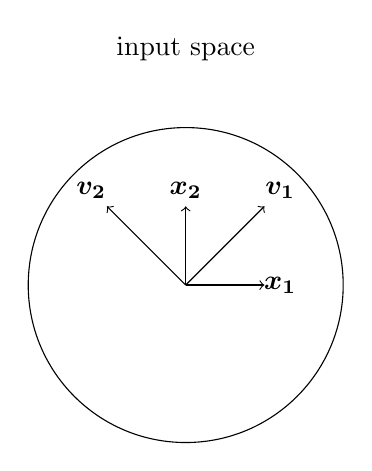
\begin{tikzpicture}
                        \node at (0, 3) {input space};

                        \node at (1.2, 0) {$\vec{x_1}$};
                        \node at (0, 1.2) {$\vec{x_2}$};
                        \node at (1.2, 1.2) {$\vec{v_1}$};
                        \node at (-1.2, 1.2) {$\vec{v_2}$};

                        \draw
                        (0, 0) edge[->] (1, 0)
                        (0, 0) edge[->] (0, 1)
                        (0, 0) edge[->] (1, 1)
                        (0, 0) edge[->] (-1, 1);
                        \draw (0, 0) circle (2);
                    \end{tikzpicture}
                    \ \ \ \ \
                    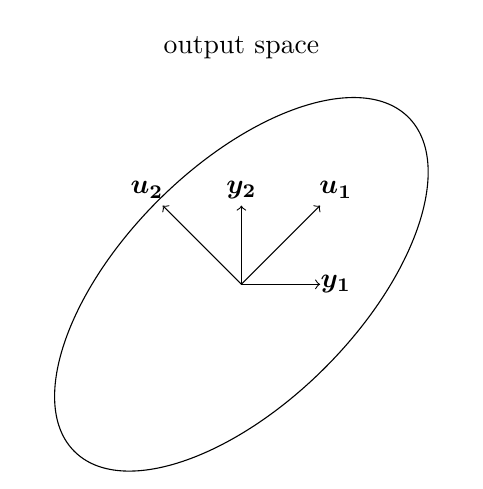
\begin{tikzpicture}
                        \node at (0, 3) {output space};

                        \node at (1.2, 0) {$\vec{y_1}$};
                        \node at (0, 1.2) {$\vec{y_2}$};
                        \node at (1.2, 1.2) {$\vec{u_1}$};
                        \node at (-1.2, 1.2) {$\vec{u_2}$};

                        \draw
                        (0, 0) edge[->] (1, 0)
                        (0, 0) edge[->] (0, 1)
                        (0, 0) edge[->] (1, 1)
                        (0, 0) edge[->] (-1, 1);
                        \draw[rotate=-45] (0, 0) circle (1.5 and 3);
                    \end{tikzpicture}
                \end{center}
                Using the same example as before, because I'm too lazy to draw this again, we see that $\vec{v_i} \mapsto \sigma_i \vec{v_i} = \vec{u_i}$.
                $\vec{v_1}$ is called the \textbf{principal component}, as it is the direction of the biggest change (since we have an ordering on $\sigma$).
                \medskip

                A brief note on why $\mat{S}\mat{S}^\top$ gives a square matrix;
                \begin{align*}
                    \mat{S} & = \begin{bmatrix}
                        \sigma_1 \\
                        & \ddots \\
                        & & \sigma_r \\
                        \hline
                        0 & \cdots & 0 \\
                        \vdots & \ddots & \vdots \\
                        0 & \cdots & 0
                    \end{bmatrix} \\
                    \mat{S}^\top & = \begin{bmatrix}[ccc|ccc]
                        \sigma_1 & & & 0 & \cdots & 0\\
                        & \ddots & & \vdots & \ddots & \vdots \\
                        & & \sigma_r & 0 & \cdots & 0
                    \end{bmatrix} \\
                    \mat{S}^\top\mat{S} & = \mat{S}\mat{S}^\top & \text{by symmetry} \\
                    & = \begin{bmatrix}
                        \sigma_1^2 \\
                        & \ddots \\
                        & & \sigma_r^2
                    \end{bmatrix}
                \end{align*}
            \subsubsection*{Cholesky Factorisation / Decomposition of Symmetric Positive Definite Matrices}
                Take a matrix $\mat{A} \in \mathbb{R}^{n \times n}$, with $\mat{A} = \mat{A}^\top$ and $\mat{A}$ is positive \violet{(semi-)}definite.
                Then the following holds
                \begin{center}
                    $\exists \mat{L} \in \mathbb{R}^{n \times n}\ [\mat{A} = \mat{L}\mat{L}^\top]$
                \end{center}
                where $\mat{L}$ is a lower triangular matrix, with all diagonal elements being positive \violet{(non-zero)};
                \begin{center}
                    $\mat{L} = \begin{bmatrix}
                        l_{1, 1} & 0 & \cdots & 0 \\
                        \times & l_{2, 2} & \ddots & \vdots \\
                        \vdots & \ddots & \ddots & 0 \\
                        \times & \cdots & \times & l_{n, n}
                    \end{bmatrix}$
                \end{center}
                This is a general result to the following, in the real numbers; $a > 0 \Rightarrow \exists l > 0\ [a = l^2]$.
                This algorithm is done with brute force, by setting $\mat{A} = (a_{i, j})$, $\mat{L} = (l_{i, j})$, and $\mat{A} = \mat{L}\mat{L}^\top$.
                The following is a simple example of this algorithm, with a $3 \times 3$ matrix;
                \begin{align*}
                    \mat{A} & = \begin{bmatrix}
                        1 & -1 & 1 \\
                        -1 & 10 & -1 \\
                        1 & -1 & 5
                    \end{bmatrix} \\
                    & = \mat{L}\mat{L}^\top \\
                    \mat{L} & = \begin{bmatrix}
                        l_{1, 1} & 0 & 0 \\
                        l_{2, 1} & l_{2, 2} & 0 \\
                        l_{3, 1} & l_{3, 2} & l_{3, 3} \\
                    \end{bmatrix} \\
                    \mat{L}^\top & = \begin{bmatrix}
                        l_{1, 1} & l_{2, 1} & l_{3, 1} \\
                        0 & l_{2, 2} & l_{3, 2} \\
                        0 & 0 & l_{3, 3}
                    \end{bmatrix}
                    \intertext{by multiplying out $\mat{L}\mat{L}^\top$, we can solve per column, starting with the first}
                    l_{1, 1}^2 & = 1 & \Rightarrow \\
                    l_{1, 1} & = 1 & \text{taking positive square root} \\
                    l_{2, 1}l_{1, 1} & = -1 & \Rightarrow \\
                    l_{2, 1} & = -1 \\
                    l_{3, 1}l_{1, 1} & = 1 & \Rightarrow \\
                    l_{3, 1} & = 1
                    \intertext{second column}
                    l_{2, 1}^2 + l_{2, 2}^2 & = 10 & \Rightarrow \\
                    l_{2, 2} & = 3 \\
                    l_{3, 1}l_{2, 1} + l_{3, 2}l_{2, 2} & = -1 & \Rightarrow\\
                    -1 + 3 l_{3, 2} & = -1 & \Rightarrow \\
                    l_{3, 2} & = 0
                    \intertext{third (final) column}
                    l_{3, 1}^2 + l_{3, 2}^2 + l_{3, 3}^2 & = 5 & \Rightarrow \\
                    1 + 0 + l_{3, 3}^2 & = 5 & \Rightarrow \\
                    l_{3, 3} & = 2
                    \intertext{setting the matrix}
                    \mat{L} & = \begin{bmatrix}
                        1 & 0 & 0 \\
                        -1 & 3 & 0 \\
                        1 & 0 & 2
                    \end{bmatrix}
                \end{align*}
                This can be used to easily solve the following;
                \begin{align*}
                    \mat{A}\vec{x} & = \vec{b} & \Leftrightarrow \\
                    \mat{L}\mat{L}^\top\vec{x} & = \vec{b} & \Leftrightarrow \\
                    \mat{L}\vec{y} & = \vec{b} & \text{let } \vec{y} = \mat{L}^\top\vec{x}
                    \intertext{This is trivial to solve with forward substitution ($y_1$ can be solved easily, then substituted into the next equation to get $y_2$ and so on) as we have a lower triangular matrix}
                    b_1 & = l_{1, 1}y_1 + 0 + \dots + 0 \\
                    b_2 & = l_{2, 1}y_1 + l_{2, 2}y_2 + 0 + \dots + 0 \\
                    b_3 & = l_{3, 1}y_1 + l_{3, 2}y_2 + l_{3, 3}y_3 + 0 + \dots + 0 \\
                    & \vdots \\
                    b_n & = l_{n, 1}y_1 + \dots + l_{n, n}y_n
                    \intertext{If $\mat{L}$ is lower triangular, then $\mat{L}^\top$ must be upper triangular, and thus can be solved with backwards substitution (such that $x_n$ is used to solve $x_{n - 1}$, and so on)}
                    \mat{U} & = \mat{L}^\top \\
                    y_n & = 0 + \dots + 0 + u_{n, n}x_n \\
                    y_{n - 1} & = 0 + \dots + 0 + u_{n - 1, n - 1}x_{n - 1} + u_{n - 1, n}x_n \\
                    & \vdots \\
                    y_1 & = u_{1, 1}x_1 + \dots + u_{1, n}x_n
                \end{align*}
            \subsubsection*{Rank-Nullity Theorem, Again}
                For a matrix $\mat{A} \in \mathbb{R}^{m \times n}$, the nullity of $\mat{A}$ (dimension of the kernel of $\mat{A}$) is $n - \text{rk}(\mat{A})$.
                To recap, a reduction to reduced row echelon form (RREF) is being in row echelon form, with the additional properties that all the pivots must be 1, and all other numbers in a column with a pivot are 0.
                \medskip

                Applying the rank-nullity theorem to $\mat{A}^\top$, where $\mat{A}^\top \in \mathbb{R}^{n \times m}$;
                \begin{align*}
                    \text{nullity}(\mat{A}^\top) + \text{rk}(\mat{A}^\top) & = m & \Rightarrow \\
                    \text{dim}(\text{ker}(\mat{A}^\top)) + \text{rk}(\mat{A}) & = m & \text{rk}(\mat{A}) = \text{rk}(\mat{A}^\top), \Rightarrow \\
                    \text{dim}(\text{ker}(\mat{A}^\top)) + \text{dim}(\text{Im}(\mat{A})) & = m & \text{rk}(\mat{A}) = \text{dim}(\text{Im}(\mat{A}))
                    \intertext{It's important to now note that these are both subspaces of $\mathbb{R}^m$}
                    \text{Im}(\mat{A}) & \subseteq \mathbb{R}^m & \text{output space of $\mat{A}$} \\
                    \text{ker}(\mat{A}^\top) & \subseteq \mathbb{R}^m \\
                \end{align*}
                Working through an example matrix, we can observe the following;
                \begin{align*}
                    \mat{A} & = \begin{bmatrix}
                        1 & 1 \\
                        1 & 0 \\
                        1 & -1
                    \end{bmatrix} \\
                    \mat{A}^\top & = \begin{bmatrix}
                        1 & 1 & 1 \\
                        1 & 0 & -1
                    \end{bmatrix} \\
                    \text{Im}(\mat{A}) & = \left\{ x_1 \begin{bmatrix}
                        1 \\ 1 \\ 1
                    \end{bmatrix} + x_2 \begin{bmatrix}
                        1 \\ 0 \\ -1
                    \end{bmatrix} : x_1, x_2 \in \mathbb{R} \right\}
                    \intertext{geometrically, Im$(\mat{A})$ is a plane going through the origin - intuitively, we can represent this with a normal (take cross product)}
                    & = \left\{ \vec{v} : \vec{v} \cdot \begin{bmatrix}
                        -1 \\ 2 \\ -1
                    \end{bmatrix} = 0 \right\} \\
                    \text{ker}(\mat{A}^\top) & = \{ \vec{w} : \mat{A}^\top\vec{w} = \vec{0} \} \\
                    \begin{bmatrix}
                        1 & 1 & 1 \\
                        1 & 0 & -1
                    \end{bmatrix} \begin{bmatrix}
                        w_1 \\ w_2 \\ w_3
                    \end{bmatrix} & = \vec{0} & \Rightarrow \\
                    \begin{bmatrix}
                        1 \\ 1 \\ 1
                    \end{bmatrix} \cdot \vec{w} & = 0 \\
                    \text{and } \begin{bmatrix}
                        1 \\ 0 \\ -1
                    \end{bmatrix} \cdot \vec{w} & = 0
                    \intertext{therefore $\vec{w}$ is orthogonal to both those matrices, hence we can take the cross product, which we already know}
                    \vec{w} & = k \begin{bmatrix}
                        -1 \\ 2 \\ -1
                    \end{bmatrix} & k \in \mathbb{R}
                \end{align*}
                We can then conclude the following;
                $$\vec{w} \in \text{ker}(\mat{A}^\top) \Leftrightarrow \vec{w} \cdot \begin{bmatrix}
                    1 \\ 1 \\ 1
                \end{bmatrix} = 0 = \vec{w} \cdot \begin{bmatrix}
                    1 \\ 0 \\ -1
                \end{bmatrix} \Leftrightarrow \forall \vec{y} \in \text{Im}(\mat{A})\ [\vec{w} \cdot \vec{y} = 0]$$
                This gives the result that $\vec{w}$ is in the null space of $\mat{A}^\top$ iff it is orthogonal to every vector in the image space of $\mat{A}$.
                \medskip

                Our conjecture is the following; $\text{ker}(\mat{A}^\top)\ \bot\ \text{Im}(\mat{A})$, which is the same as saying
                \begin{center}
                    $\vec{v} \in \text{ker}(\mat{A}^\top) \Leftrightarrow \forall \vec{y} \in \text{Im}(\mat{A})\ [\vec{y} \cdot \vec{v} = 0]$
                \end{center}
                This can be proven generally as follows;
                \begin{align*}
                    & \vec{v} \in \text{ker}(\mat{A}^\top) \\
                    \Leftrightarrow\ & \mat{A}^\top\vec{v} = \vec{0} & \text{by definition of the null space / kernel} \\
                    \Leftrightarrow\ & \forall i \in [1, n]\ [\vec{a_i} \cdot \vec{v} = 0] & (1) \\
                    \Leftrightarrow\ & \forall \vec{x} \in \mathbb{R}^n\ \left[\left(\summation{i = 1}{n} x_i \vec{a_i} \right) \cdot \vec{v} = 0\right] & \text{generalise to any linear combination} \\
                    \Leftrightarrow\ & \vec{y} \in \text{Im}(\mat{A})\ [\vec{y} \cdot \vec{v} = 0] & \blacksquare
                \end{align*}
                \begin{enumerate}[(1)]
                    \itemsep0em
                    \item row $i$ of $\mat{A}^\top \in \mathbb{R}^{n \times m}$ is the same as column $i$ of $\mat{A} \in \mathbb{R}^{m \times n}$, transposed, and all of the components must become 0
                \end{enumerate}
                We say that $\mathbb{R}^m$ is the direct sum of $\text{ker}(\mat{A}^\top)$ and $\text{Im}(\mat{A})$.
                We can get the following result, following what was proven earlier;
                \begin{center}
                    $\vec{v} \in \text{Im}(\mat{A}) \land \vec{v} \in \text{ker}(\mat{A}^\top) \Leftrightarrow \vec{v} \cdot \vec{v} = 0 \Leftrightarrow \vec{v} = \vec{0}$
                \end{center}
                We want to prove the result for any vector $\vec{x} \in \mathbb{R}^m$, there exists a unique vector $\vec{x_r} \in \text{Im}(\mat{A})$ and $\vec{x_n} \in \text{ker}(\mat{A}^\top)$, such that $\vec{x} = \vec{x_r} + \vec{x_n}$, or formally;
                \begin{center}
                    $\forall \vec{x} \in \mathbb{R}^m\ \exists ! \vec{x_r} \in \text{Im}(\mat{A}), \vec{x_n} \in \text{ker}(\mat{A}^\top)\ [\vec{x} = \vec{x_r} + \vec{x_n}]$
                \end{center}
                By taking the union of a basis of $\text{Im}(\mat{A})$, let it be $(\vec{v_1}, \dots, \vec{v_r})$, and a basis of $\text{ker}(\mat{A}^\top)$, let it be $(\vec{v_{r + 1}}, \dots, \vec{v_m})$, we get a basis of $\mathbb{R}^m$: $(\vec{v_1}, \dots, \vec{v_r}, \vec{v_{r + 1}}, \dots, \vec{v_m})$.
                This gives us the following result;
                $$\vec{x} \in \mathbb{R}^m = \summation{i = 1}{m} x_i \vec{v_i} = \underbrace{\summation{i = 1}{r} x_i \vec{v_i}}_{\in \text{Im}(\mat{A})} + \underbrace{\summation{i = r + 1}{m} x_i \vec{v_i}}_{\in \text{ker}(\mat{A}^\top)} = \vec{x_r} + \vec{x_n}$$
                In order to prove uniqueness, we assume $\vec{x} = \violet{\vec{x_r} + \vec{x_n} = \vec{x_r^\prime} + \vec{x_n^\prime}}$.
                The \violet{violet} part only holds iff $\vec{x_r} - \vec{x_r^\prime} = \vec{x_n^\prime} - \vec{x_n}$.
                As they are both in their respective subspaces of $\text{Im}(\mat{A})$ and $\text{ker}(\mat{A}^\top)$, they must both be $\vec{0}$, as shown above.
                This gives the result $\vec{x_r} = \vec{x_r^\prime} \land \vec{x_n} = \vec{x_n^\prime}$, hence proving uniqueness.
        \subsection*{5th February 2020}
            \subsubsection*{Positive Definiteness}
                The conditions for positive definiteness ($\forall \vec{x} \neq \vec{0}\ [\vec{x}^\top\mat{A}\vec{x} > 0]$) of $\mat{A}$ are as follows ;
                \begin{itemize}
                    \itemsep0em
                    \item all diagonal elements of $\mat{A}$ must be $> 0$
                        \medskip

                        Take $\vec{x} = \vec{e_i}$, which is all 0, other than the $i^\text{th}$ entry being 1.
                        Then $\vec{e_i}^\top\mat{A}\vec{e_i} = a_{i, i}$, which has to be greater than 0.
                    \item all principal minors of $\mat{A}$ must be positive definite.
                        \medskip

                        For $1 \leq k \leq n$, $\mat{A^{(k)}} \in \mathbb{R}^{k \times k}$ denotes the top left square submatrix of $\mat{A}$.
                        \begin{align*}
                            \vec{x} & = \begin{bmatrix}
                                \vec{y} \\ \vec{0}
                            \end{bmatrix} & \text{where } \vec{y} \in \mathbb{R}^k, \vec{0} \in \mathbb{R}^{n - k} \\
                            \vec{x}^\top\mat{A}\vec{x} & = \begin{bmatrix}
                                \vec{y} \\ \vec{0}
                            \end{bmatrix}^\top \mat{A} \begin{bmatrix}
                                \vec{y} \\ \vec{0}
                            \end{bmatrix} \\
                            & = \vec{y}^\top\mat{A^{(k)}}\vec{y}
                        \end{align*}
                        So for any $\vec{y} \neq \vec{0}$, $\vec{x} \neq \vec{0}$, thus $\vec{y}^\top\mat{A^{(k)}}\vec{y} > 0 \Leftrightarrow \vec{x}^\top\mat{A}\vec{x} > 0$
                    \item $| a_{i, j} | < \max \{ a_{i, i}, a_{j, j} \}$
                        \medskip

                        For any entry not on the diagonal, there are two corresponding entries on the diagonal (one corresponding to the row, the other to the column);
                        \begin{align*}
                            \mat{A} & = \begin{bmatrix}
                                \ddots & & & & \\
                                & a_{i, i} & \cdots & a_{i, j} & \\
                                & & \ddots & \vdots & \\
                                & & & a_{j, j} & \\
                                & & & & \ddots
                            \end{bmatrix} \\
                            \text{take } \vec{x} & = \vec{e_i} + \vec{e_j} \\
                            \vec{x}^\top\mat{A}\vec{x} & =(\vec{e_i} \pm \vec{e_j})^\top\mat{A}(\vec{e_i} \pm \vec{e_j}) \\
                            & = \left(\vec{e_i}^\top \pm \vec{e_j}^\top\right)\mat{A}(\vec{e_i} \pm \vec{e_j}) \\
                            & = \vec{e_i}^\top\mat{A}\vec{e_i} + \vec{e_j}^\top\mat{A}\vec{e_j} \pm \vec{e_i}^\top\mat{A}\vec{e_j} \pm \vec{e_j}^\top\mat{A}\vec{e_i} \\
                            & = a_{i, i} + a_{j, j} \pm 2 a_{i, j} & \text{$\mat{A}$ is symmetric} \\
                            & > 0 & \Rightarrow \\
                            -a_{i, j} & < \frac{a_{i, i} + a_{j, j}}{2} & \text{diagonal terms are positive} \\
                            \text{or } a_{i, j} & < \frac{a_{i, i} + a_{j, j}}{2} & \Rightarrow \\
                            | a_{i, j} | & < \max \{ a_{i, i}, a_{j, j} \}
                        \end{align*}
                    \item all positive eigenvalues
                \end{itemize}
                For an example, take the following;
                \begin{align*}
                    \mat{A} & = \begin{bmatrix}
                        1 & -1 & 3 \\
                        -1 & 10 & -1 \\
                        -3 & -1 & 2
                    \end{bmatrix}
                \end{align*}
                However, we see that $| -3 | = 3 > 2 = \max \{1, 2\}$, hence $\mat{A}$ is not positive definite
            \subsubsection*{Least Square Method}
                For a matrix $\mat{A} \in \mathbb{R}^{m \times n}$, where $n$ is commonly the dimension of the data, and $m$ the number of samples (such that each row is an entry), we can write $\mat{A}$ as;
                \begin{center}
                    $\mat{A} = \begin{bmatrix}
                        \vec{a^1} \\ \vec{a^2} \\ \vdots \\ \vec{a^m}
                    \end{bmatrix}$ (all rows)
                \end{center}
                The goal of the LSM is to find a $\vec{x} \in \mathbb{R}^n$, such that $|| \mat{A}\vec{x} - \vec{b} ||_2$ is minimised (which is equivalent to minimising $|| \mat{A}\vec{x} - \vec{b} ||_2^2$, as it is positive).
                From previous results, we can take $\vec{b} = \vec{b_r} + \vec{b_n}$, therefore we can minimise the following;
                \begin{align*}
                    || \mat{A}\vec{x} - \vec{b_r} - \vec{b_n} ||_2^2 & = ((\mat{A}\vec{x} - \vec{b_r}) - \vec{b_n}) \cdot ((\mat{A}\vec{x} - \vec{b_r}) - \vec{b_n}) \\
                    & = (\mat{A}\vec{x} - \vec{b_r}) \cdot (\mat{A}\vec{x} - \vec{b_r}) + \vec{b_n} \cdot \vec{b_n} - 2 \overbrace{(\mat{A}\vec{x} - \vec{b_r})}^{\in \text{Im}(\mat{A})} \cdot \hspace{-0.4cm} \underbrace{\vec{b_n}}_{\in \text{ker}(\mat{A}^\top)} & (1) \\
                    & = (\mat{A}\vec{x} - \vec{b_r}) \cdot (\mat{A}\vec{x} - \vec{b_r}) + \vec{b_n} \cdot \vec{b_n} & (2)
                \end{align*}
                \begin{enumerate}[(1)]
                    \itemsep0em
                    \item the dot product is bilinear in both variables, hence we can expand out
                    \item range space of $\mat{A}$ is perpendicular to the null space of $\mat{A}^\top$, hence the dot product is 0
                \end{enumerate}
                Therefore, we want to minimise $(\mat{A}\vec{x} - \vec{b_r}) \cdot (\mat{A}\vec{x} - \vec{b_r}) + \vec{b_n} \cdot \vec{b_n}$.
                However, we have no control over $\vec{b_n}$, therefore we want to solve for $\mat{A}\vec{x} = \vec{b_r}$.
                This will always have a solution, as $\vec{b_r} \in \text{Im}(\mat{A})$, which means that such a $\vec{x}$ exists by definition of the range space.
                We then claim the following;
                \begin{center}
                    $\mat{A}\vec{x} = \vec{b_r} \Leftrightarrow \mat{A}^\top\mat{A}\vec{x} = \mat{A}^\top\mat{b}$
                \end{center}
                Therefore, if the left hand side of the double implication has a solution, which we know it does, then the right hand side must also have a solution.
                The proof for this is done in both directions;
                \begin{align*}
                    \intertext{proving "$\Rightarrow$"}
                    \text{suppose } \mat{A}\vec{x} & = \vec{b_r} & \Rightarrow \\
                    \violet{\mat{A}^\top\mat{A}\vec{x}} & = \mat{A}^\top\vec{b_r} & \text{pre-multiply} \\
                    & = \mat{A}^\top(\vec{b_r} + \vec{b_n}) & \text{in null space, hence } \mat{A}^\top\vec{b_n} = \vec{0} \\
                    & = \violet{\mat{A}^\top\vec{b}} & \blacksquare
                    \intertext{proving "$\Leftarrow$"}
                    \text{suppose } \mat{A}^\top\mat{A}\vec{x} & = \mat{A}^\top\vec{b} & \Rightarrow \\
                    \mat{A}^\top\mat{A}\vec{x} - \mat{A}^\top(\vec{b_r} + \vec{b_n}) & = \vec{0} & \Rightarrow \\
                    \mat{A}^\top(\mat{A}\vec{x} - \vec{b_r} - \vec{b_n}) & = \vec{0} & \Rightarrow \\
                    \mat{A}\vec{x} - \vec{b_r} - \vec{b_n} & \in \text{ker}(\mat{A}^\top) & \text{property of adding in subspace}, \Rightarrow \\
                    \mat{A}\vec{x} - \vec{b_r} & \in \text{ker}(\mat{A}^\top) & \text{and} \\
                    \mat{A}\vec{x} - \vec{b_r} & \in \text{Im}(\mat{A}^\top) & \text{adding two elements of the range space}, \Rightarrow \\
                    \mat{A}\vec{x} - \vec{b_r} & = \vec{0} & \Rightarrow \\
                    \violet{\mat{A}\vec{x}} & = \violet{\vec{b_r}} & \blacksquare
                \end{align*}
                An example of using this is as follows (note that $\mat{A}\vec{x} = \vec{b}$ is inconsistent);
                \begin{align*}
                    \mat{A} & = \begin{bmatrix}
                        2 & 2 \\
                        1 & 2 \\
                        2 & 0
                    \end{bmatrix} \\
                    \vec{b} & = \begin{bmatrix}
                        0 \\ 5 \\ -1
                    \end{bmatrix}
                    \intertext{find $\vec{x}$ such that $\mat{A}\vec{x} = \vec{b_r}$}
                    \mat{A}^\top\mat{A}\vec{x} & = \mat{A}^\top\vec{b} & \Rightarrow \\
                    \begin{bmatrix}
                        9 & 6 \\
                        6 & 8
                    \end{bmatrix} \begin{bmatrix}
                        x_1 \\ x_2
                    \end{bmatrix} & = \begin{bmatrix}
                        2 & 1 & 2 \\
                        2 & 2 & 0
                    \end{bmatrix} \begin{bmatrix}
                        0 \\ 5 \\ -1
                    \end{bmatrix} \\
                    & = \begin{bmatrix}
                        3 \\ 10
                    \end{bmatrix}
                    \intertext{we know this is positive definite, and therefore there is a solution}
                    x_1 & = -1 \\
                    x_2 & = 2
                \end{align*}
        \subsection*{6th February 2020}
            \subsubsection*{Using Cholesky Decomposition for LSM}
                While it's easy in some cases to solve with an inverse, we have a symmetric positive definite matrix in $\mat{A}^\top\mat{A}$.
                Therefore we have the following steps;
                \begin{itemize}
                    \itemsep0em
                    \item goal is to solve $\mat{A}^\top\mat{A}\vec{x} = \mat{A}^\top\vec{b}$
                    \item let $\mat{A}^\top\mat{A} = \mat{L}\mat{L}^\top$, therefore we have $\mat{L}\mat{L}^\top\vec{x} = \mat{A}^\top\vec{b}$
                    \item let $\vec{y} = \mat{L}^\top\vec{x}$
                    \item find $\vec{y}$ with forward substitution in $\mat{L}\vec{y} = \mat{A}^\top\vec{b}$
                    \item find $\vec{x}$ with backward substitution in $\vec{y} = \mat{L}^\top\vec{x}$
                \end{itemize}
            \subsubsection*{First Application (Linear Regression) + Example}
                A simple application for this is to consider $m$ samples of pairs $(a_i, b_i)$.
                We want to find an affine line $y = s_1 x + s_0$, such that;
                \begin{center}
                    $\summation{i = 1}{m} e_i^2$ is minimised, where the error term $e_i = | (s_1 a_i + s_0) - b_i |$
                \end{center}
                In this case, we only have two unknowns, and therefore we can write the following;
                \begin{align*}
                    \mat{A} & = \begin{bmatrix}
                        1 & a_1 \\
                        1 & a_2 \\
                        \vdots & \vdots \\
                        1 & a_m
                    \end{bmatrix} \\
                    \vec{b} & = \begin{bmatrix}
                        b_1 \\ b_2 \\ \vdots \\ b_m
                    \end{bmatrix} \\
                    \vec{z} & = \begin{bmatrix}
                        s_0 \\ s_1
                    \end{bmatrix} \\
                    \mat{A}\vec{z} & = \vec{b} & \Rightarrow \displaybreak \\
                    \begin{bmatrix}
                        1 & a_1 \\
                        1 & a_2 \\
                        \vdots & \vdots \\
                        1 & a_m
                    \end{bmatrix} \begin{bmatrix}
                        s_0 \\ s_1
                    \end{bmatrix} & = \begin{bmatrix}
                        s_0 + a_1 s_1 \\
                        s_0 + a_2 s_1 \\
                        \vdots \\
                        s_0 + a_m s_1
                    \end{bmatrix} \\
                    & = \begin{bmatrix}
                        b_1 \\ b_2 \\ \vdots \\ b_m
                    \end{bmatrix}
                \end{align*}
                However, being able to solve it exactly is unlikely, especially for large datasets.
                In a real example, we have the following;
                \begin{align*}
                    (a_1, b_1) & = (1, 6), (2, 5), (3, 7), (4, 10) \\
                    \mat{A} & = \begin{bmatrix}
                        1 & 1 \\
                        1 & 2 \\
                        1 & 3 \\
                        1 & 4
                    \end{bmatrix} \\
                    \mat{b} & = \begin{bmatrix}
                        6 \\ 5 \\ 7 \\ 10
                    \end{bmatrix} \\
                    \mat{A}^\top\mat{A} & = \begin{bmatrix}
                        1 & 1 & 1 & 1 \\
                        1 & 2 & 3 & 4
                    \end{bmatrix} \begin{bmatrix}
                        1 & 1 \\
                        1 & 2 \\
                        1 & 3 \\
                        1 & 4
                    \end{bmatrix} \\
                    & = \begin{bmatrix}
                        4 & 10 \\
                        10 & 30
                    \end{bmatrix} \\
                    \mat{A}^\top\vec{b} & = \begin{bmatrix}
                        1 & 1 & 1 & 1 \\
                        1 & 2 & 3 & 4
                    \end{bmatrix} \begin{bmatrix}
                        6 \\ 5 \\ 7 \\ 10
                    \end{bmatrix} \\
                    & = \begin{bmatrix}
                        28 \\ 77
                    \end{bmatrix}
                    \intertext{by doing Gaussian elimination, we get the following results}
                    s_0 & = \frac{7}{2} \\
                    s_1 & = \frac{7}{5}
                \end{align*}
                \begin{center}
                    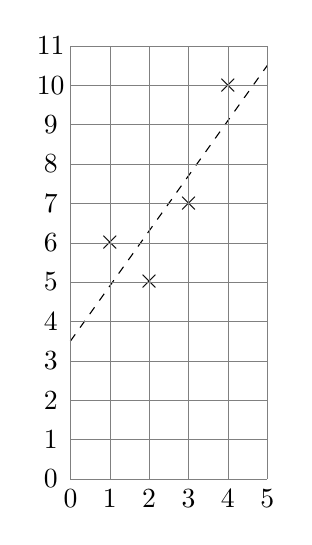
\begin{tikzpicture}[x=0.5cm, y=0.5cm]
                        \node (p1) at (1, 6) {$\times$};
                        \node (p2) at (2, 5) {$\times$};
                        \node (p3) at (3, 7) {$\times$};
                        \node (p4) at (4, 10) {$\times$};

                        \draw[dashed] (0, 3.5) -- (5, 10.5);

                        \draw[step=1, line width=0.1, black!50!white] (0,0) grid (5,11);

                        \foreach \xtick in {0,...,5} {\pgfmathsetmacro\result{\xtick} \node at (\xtick,-0.5) {\pgfmathprintnumber{\result}}; }
                        \foreach \ytick in {0,...,11} {\pgfmathsetmacro\result{\ytick} \node at (-0.5, \ytick) {\pgfmathprintnumber{\result}}; }
                    \end{tikzpicture}
                \end{center}
            \subsubsection*{Higher Dimensions}
                In order to generalise this to higher dimensions, for each $(a_i, b_i)$, we now have a vector $\vec{a_i} \in \mathbb{R}^n$, and a scalar $b_i \in \mathbb{R}$, for $i = 1, \dots, m$.
                The affine line is now no longer as simple, and is therefore written as;
                \begin{center}
                    $y = \vec{x}^\top\vec{s} + s_0 = \vec{x} \cdot \vec{s} + s_0 = s_0 + \summation{j = 1}{n} x_j s_j $, where $\vec{s} \in \mathbb{R}^n$, and $s_0 \in \mathbb{R}$.
                \end{center}
                Setting this out, we have the following;
                \begin{align*}
                    \vec{a_i} & = \begin{bmatrix}
                        a_{i, 1} \\ \vdots \\ a_{i, n}
                    \end{bmatrix} & \text{for } i = 1, \dots, m \\
                    \mat{A} & = \begin{bmatrix}
                        1 & a_{1, 1} & \cdots & a_{1, n} \\
                        1 & a_{2, 1} & \cdots & a_{2, n} \\
                        \vdots & \vdots & \ddots & \vdots \\
                        1 & a_{2, 1} & \cdots & a_{m, n}
                    \end{bmatrix} \\
                    \vec{b} & = \begin{bmatrix}
                        b_1 \\ b_2 \\ \vdots \\ b_m
                    \end{bmatrix} \\
                    \vec{z} & = \begin{bmatrix}
                        s_0 \\ \vec{s}
                    \end{bmatrix} & \vec{s} \in \mathbb{R}^n
                \end{align*}
            \subsubsection*{Second Application (Polynomial Regression)}
                Another application of this is to suppose data is $(y_i, t_i)$, where $y_i \in \mathbb{R}$ and $t_i \in \mathbb{R}$ (considered as "time" - but is any continuous variable).
                We hypothesise the following;
                \begin{center}
                    $y(t) = \summation{j = 1}{n} P_j f_j(t)$
                \end{center}
                where $P_j$s are the parameters of the model, and $f_j$s are basic functions, for \textbf{example}; $f_1(t) = 1, f_2(t) = t, \dots, f_n(t) = t^{n - 1}$.
                This is called \textbf{polynomial regression}.
                We know (we're given) $f_j$s, but we want to find the $P_j$s.
                \begin{align*}
                    \mat{A}\vec{x} & = \vec{y} \\
                    \mat{A} & = (a_{i, j}) \\
                    a_{i, j} & = f_j(t_i) \\
                    \vec{x} & = \begin{bmatrix}
                        P_1 \\ P_2 \\ \vdots \\ P_m
                    \end{bmatrix}
                \end{align*}
                An example of this is to determine height ($h$), and the coefficient of gravity ($g$).
                We hypothesise that the distance with respect to time, away from the start, is
                $$y(t) = h - g \frac{t^2}{2}$$
                We assume that $h$ and $g$ are the unknown parameters, and define the basic functions as follows (note that the pairs $(y_i, t_i)$ can be obtained with experiments);
                \begin{align*}
                    f_1(t) & = 1 \\
                    f_2(t) & = -\frac{t^2}{2} \\
                    \mat{A} & = \begin{bmatrix}
                        1 & -\frac{t_1^2}{2} \\
                        \vdots & \vdots \\
                        1 & -\frac{t_m^2}{2}
                    \end{bmatrix} \\
                    \vec{x} & = \begin{bmatrix}
                        h \\ g
                    \end{bmatrix} \\
                    \vec{y} & = \begin{bmatrix}
                        y_1 \\ \vdots \\ y_m
                    \end{bmatrix}
                \end{align*}
                This can now be solved with the standard LSM.
            \subsubsection*{QR Decomposition}
                We define $\mat{Q} \in \mathbb{R}^{m \times n}$ to be an orthogonal matrix if $\mat{Q} = [\vec{q_1}, \dots, \vec{q_n}]$, the column vectors are unit vectors with respect to the $\ell_2$-norm, and are pairwise orthogonal.
                This is only possible if $n \leq m$.
                It's important to note that $\mat{Q}^\top\mat{Q} = \mat{I}_n$, and $\mat{Q}\mat{Q}^\top = \mat{I}_m$.
                \medskip

                The goal is to find $\mat{Q}$ and $\mat{R}$ such that $\mat{A} = \mat{Q}\mat{R}$, where $\mat{Q}$ is an orthogonal matrix, and $\mat{R}$ is an upper triangular matrix.
                It's trivial to see that $\mat{R} = \mat{Q}^\top\mat{A}$, due to the previously mentioned property.
                This is used to easily solve the following (since $\mat{R}$ is upper triangular, we can employ backward substitution);
                \begin{center}
                    $\mat{A}\vec{x} = \vec{b} \Rightarrow \mat{Q}\mat{R}\vec{x} = \vec{b} \Rightarrow \mat{R}\vec{x} = \mat{Q}^\top\vec{b}$
                \end{center}
            \subsubsection*{Gram-Schmidt Process}
                Suppose we have a set of linearly independent vectors $\vec{a_1}, \dots, \vec{a_n} \in \mathbb{R}^m$.
                The Gram-Schmidt process is as follows;
                \begin{align*}
                    \vec{u_1} & = \vec{a_1} & \vec{e_1} & = \frac{\vec{u_1}}{|| \vec{u_1} ||} \\
                    \vec{u_2} & = \vec{a_2} - (\vec{e_1} \cdot \vec{a_2}) \vec{e_1} & \vec{e_2} & = \frac{\vec{u_2}}{|| \vec{u_2} ||} \\
                    \vec{u_3} & = \vec{a_3} - (\vec{e_1} \cdot \vec{a_3}) \vec{e_1} - (\vec{e_2} \cdot \vec{a_3}) \vec{e_2} & \vec{e_2} & = \frac{\vec{u_3}}{|| \vec{u_3} ||} \\
                    & \vdots & & \vdots \\
                    \vec{u_n} & = \vec{a_n} - \summation{j = 1}{n - 1} (\vec{e_j} \cdot \vec{a_n}) \vec{e_j} & \vec{e_n} & = \frac{\vec{u_n}}{|| \vec{u_n} ||}
                \end{align*}
                Geometrically, we can visualise it as the following;
                \begin{center}
                    \begin{tikzpicture}
                        \node at (3.3, -0.3) {$\vec{a_1} = \vec{u_1}$};
                        \node at (1.3, -0.3) {$\vec{e_1}$};
                        \node at (2.3, 2.3) {$\vec{a_2}$};
                        \node at (-0.3, 2.3) {$\vec{u_2}$};
                        \node at (-0.3, 1.3) {$\vec{e_2}$};

                        \draw
                        (0, 0) edge[->] (3, 0)
                        (0, 0) edge[->] (2, 2)
                        (0, 0) edge[->] (0, 2)
                        (0, 0) edge[->] (0, 1)
                        (0, 0) edge[->] (1, 0);

                        \draw[dashed] (2, 2) -- (2, 0);
                    \end{tikzpicture}
                \end{center}
                In general, for $1 \leq j \leq n$, we have
                \begin{center}
                    $\vec{a_j} = (\vec{e_1} \cdot \vec{a_j}) \vec{e_1} + (\vec{e_2} \cdot \vec{a_j}) \vec{e_2} + \dots + (\vec{e_j} \cdot \vec{a_j}) \vec{e_j}$
                \end{center}
            \subsubsection*{First Method for QR Decomposition (Gram-Schmidt Process)}
                Take a matrix $\mat{A} \in \mathbb{R}^{m \times n}$, where $\mat{A} = [\vec{a_1}, \dots, \vec{a_n}]$, assuming that $\vec{a_1}, \dots, \vec{a_n}$ are linearly independent.
                We then apply Gram-Schmidt to $\vec{a_1}, \dots, \vec{a_n}$ as described above to get $\mat{Q}_0 = (\vec{e_1}, \dots, \vec{e_n})$, where.
                Note that for $1 \leq j \leq n$, $\vec{e_j} \cdot \vec{e_j} = 1$, and for $j \neq k$, $\vec{e_j} \cdot \vec{e_k} = 0$.
                Let $\mat{Q} = [\vec{e_1}, \dots, \vec{e_n}]$, which is orthogonal.
                While we can see that $\mat{R} = \mat{Q}^\top\mat{A}$, we can write this as;
                \begin{center}
                    $\mat{R} = \begin{bmatrix}
                        \vec{e_1} \cdot \vec{a_1} & \vec{e_1} \cdot \vec{a_2} & \vec{e_1} \cdot \vec{a_3} & \cdots & \vec{e_1} \cdot \vec{a_n} \\
                        & \vec{e_2} \cdot \vec{a_2} & \vec{e_2} \cdot \vec{a_3} & \cdots & \vec{e_2} \cdot \vec{a_n} \\
                        & & \vec{e_3} \cdot \vec{a_3} & \cdots & \vec{e_3} \cdot \vec{a_n} \\
                        & & & \ddots & \vdots \\
                        & & & & \vec{e_n} \cdot \vec{a_n}
                    \end{bmatrix} \in \mathbb{R}^{n \times n}$
                \end{center}
                We claim that the diagram below is valid when $\mat{A}$ represents the linear map $f: \mathbb{R}^n \to \mathbb{R}^m$, in the standard basis.
                \begin{center}
                    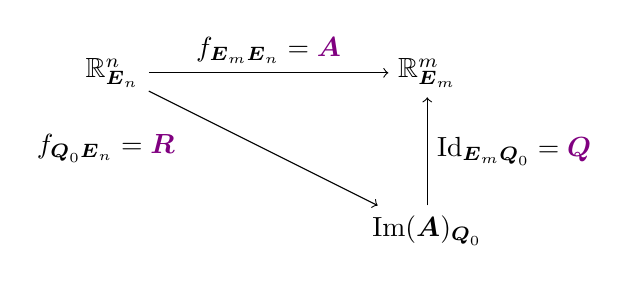
\begin{tikzpicture}
                        \node (rn) at (0, 0) {$\mathbb{R}_{\mat{E}_n}^n$};
                        \node (rm) at (4, 0) {$\mathbb{R}_{\mat{E}_m}^m$};
                        \node (im) at (4, -2) {$\text{Im}(\mat{A})_{\mat{Q}_0}$};

                        \draw
                        (rn) edge[->] node[above]{$f_{\mat{E}_m\mat{E}_n} = \violet{\mat{A}}$} (rm)
                        (rn) edge[->] node[left]{$f_{\mat{Q}_0\mat{E}_n} = \violet{\mat{R}}\hspace{1cm}$} (im)
                        (im) edge[->] node[right]{$\text{Id}_{\mat{E}_m\mat{Q}_0} = \violet{\mat{Q}}$} (rm);
                    \end{tikzpicture}
                \end{center}
\end{document}